\documentclass[12pt,english]{article}
\usepackage{geometry}
\geometry{verbose,letterpaper,tmargin=2.54cm,bmargin=2.54cm,lmargin=2.54cm,rmargin=2.54cm}
\geometry{letterpaper}
\usepackage{amssymb}
\usepackage{amsmath}
\usepackage{amsfonts}
\usepackage{graphicx}
\usepackage{setspace}
\usepackage[round]{natbib}
\bibpunct{(}{)}{;}{a}{}{;}
\textheight 22.0cm
\usepackage{lineno}
\usepackage{xcolor}
%\renewcommand\linenumberfont{\normalfont\tiny\sffamily\color{gray}}
\usepackage{booktabs}
\usepackage{cite}
\usepackage[originalparameters]{ragged2e}
\usepackage{array}
%\usepackage{mathptmx}

\newlabel{f:flowchart}{{1}{999}}
\newlabel{f:curves}{{2}{999}}
\newlabel{f:ts}{{3}{999}}
\newlabel{f:sp}{{4}{999}}
\newlabel{f:n}{{5}{999}}
\newlabel{f:squeeze}{{6}{999}}

\newcommand{\somR}{Appendix A}
\newcommand{\somparam}{Appendix B}
\newcommand{\somstray}{Appendix C}
\newcommand{\somsens}{Appendix D}
\newcommand{\somcor}{Appendix E}
\newcommand{\somts}{Appendix F}

% SOM:
\newlabel{t:pars}{{B1}{2}}
\newlabel{f:stray}{{C1}{3}}
\newlabel{f:eg-sens}{{D1}{4}}
\newlabel{f:ret-corr}{{E1}{5}}
\newlabel{f:eg-sp-arma-full}{{F1}{6}}
\newlabel{f:eg-sp-arma-half}{{F2}{7}}
\newlabel{f:eg-sp-linear-full}{{F3}{8}}
\newlabel{f:eg-sp-linear-half}{{F4}{9}}
\newlabel{f:eg-n-arma-two}{{F5}{10}}
\newlabel{f:eg-n-arma-sixteen}{{F6}{11}}
\newlabel{f:eg-n-linear-two}{{F7}{12}}
\newlabel{f:eg-n-linear-sixteen}{{F8}{13}}
\newlabel{f:eg-n-squeeze-two}{{F9}{14}}
\newlabel{f:eg-n-squeeze-twelve}{{F10}{15}}


\DeclareGraphicsExtensions{.pdf}

\widowpenalty=10000
\clubpenalty=10000

%\usepackage{titlesec}
%\titlespacing\section{0pt}{6pt plus 4pt minus 2pt}{-8pt plus 2pt minus 2pt}
%\titlespacing\subsection{0pt}{6pt plus 4pt minus 2pt}{-8pt plus 2pt minus 2pt}

\title{Portfolio conservation of metapopulations under\\climate change}

\author{
Sean C. Anderson$^{1\ast}$ \and Jonathan W. Moore$^{1,2}$ \and Michelle M. McClure$^3$ \and
Nicholas K. Dulvy$^1$ \and Andrew B. Cooper$^2$
}
\date{}

% remove numbers in front of sections:
\makeatletter
\renewcommand\@seccntformat[1]{}
\makeatother

\hyphenation{meta-pop-ulation meta-pop-ulations sub-pop-ulations sub-pop-ulation e-con-o-mist en-vi-ron-men-tal pri-or-i-ti-za-tion}

%\newcommand{\R}[1]{\label{#1}\linelabel{#1}}
%\newcommand{\lr}[1]{line~\lineref{#1}}

\begin{document}
\raggedright

\begin{spacing}{1.1}
\setlength\parskip{0.11in}
\setlength\parindent{0in}
%\include{response}
\setlength\parskip{0in}
\end{spacing}

\setcounter{page}{1}
\linenumbers

%\modulolinenumbers[2]
\begin{spacing}{1.9}
%\begin{spacing}{1.2}
\setlength{\parindent}{0.9cm}

\maketitle

%\section{Portfolio conservation of metapopulations under climate change}

\setlength{\parskip}{6pt} \setlength{\parindent}{0cm}

Sean C. Anderson\textsuperscript{1*}, Jonathan W. Moore\textsuperscript{1}, Trevor A. Branch?, Nicholas K. Dulvy\textsuperscript{1}, Michelle M. McClure?, Andrew B. Cooper\textsuperscript{2} (Authors and order to be discussed)

\textsuperscript{1}Department of Biological Sciences, Simon Fraser University, Burnaby BC, V5A 1S6, Canada

\textsuperscript{2}School of Resource and Environmental Management, Simon Fraser University, Burnaby, BC, V5A 1S6, Canada

\emph{Statement of authorship}: SCA, JWM, NKD, and ABC designed the analyses. SCA wrote the simulation code, analyzed the results, and wrote the first draft of the manuscript. All authors contributed substantially to revisions.

\emph{Running title}: Portfolio conservation of metapopulations (maximum 45 characters)

\emph{Keywords}: biocomplexity, Modern Portfolio Theory, portfolio effect, prioritization, resource management, range contraction, response diversity, risk assessment, salmon, stochastic simulation (maximum 10)

\emph{Type of article}: Letters

\emph{Words in abstract and main text}: (maximum 150, 5000)

\emph{Number of references}: (maximum 50)

\emph{Number of tables and figures}: 1, 5

\textsuperscript{*}Corresponding author: Sean C. Anderson; Department of Biological Sciences, Simon Fraser University, Burnaby BC, V5A 1S6; Phone: 1-778-782-3989; E-mail: sean\_anderson@sfu.ca

\setlength{\parskip}{2pt} \setlength{\parindent}{16pt}

\section{Abstract}

Managing risk is fundamental to the conservation of an endangered species. When an endangered species exists as a metapopulation, we typically manage risk at the subpopulation level. However, a portfolio approach might consider how conservation affects the ``weight'' of each population in a metapopulation ``portfolio''. Here we ask how such a portfolio approach can inform conservation priorities for metapopulations in a changing world. We develop a salmon metapopulation simulation in which population-specific productivity is driven by spatially-distributed thermal tolerance and patterns of short- and long-term environmental change. We then implement spatial conservation strategies that control subpopulation carrying capacities and evaluate the salmon portfolios along risk-return axes. We show that conserving response diversity minimizes risk given environmental stochasticity and ensures persistence given long-term environmental change. Further, conserving more subpopulations minimizes risk regardless of response diversity distribution. These findings have important implications for how we prioritize metapopulation conservation and emphasize the importance of conserving the processes that promote response diversity.

\section{Introduction}

Managing risk is fundamental to conserving endangered species \citep{burgman2005, iucn2009}. When an endangered species exists as a metapopulation, we can manage risk at two levels: at the population level or at the metapopulation level. Typically we treat sources of risk at the metapopulation level as exogenous and manage risk at the population level by manipulating hunting or fishing levels, implementing reserves, or improving connectivity \citep[e.g.][]{akcakaya2007}.

The management of financial portfolios provides another way of considering risk \citep{figge2004, koellner2006, ando2012}. Economists consider the risk and performance of a financial portfolio based on the weighting of individual investments (called assets) that make up the portfolio. Modern Portfolio Theory proposes that a set of portfolios maximizes expected return for a level of risk or minimizes risk for a level of return \citep{markowitz1952, markowitz1959}. Similarly, expected growth rate and variance of a metapopulation is a function of the variance, covariance, and size of the individual populations \citep{moore2010}. A portfolio approach to managing risk for a metapopulation might therefore consider how conservation actions affect the weight of each population in a metapopulation portfolio.

Managing Pacific salmon under the uncertainty of climate change is an ideal scenario to consider through the lens of portfolio theory for three reasons. (1) Pacific salmon form metapopulations \citep{rieman2000, schtickzelle2007} and we can consider, for example, the metapopulation in a river-catchment as a portfolio and the stream populations as assets \citep{schindler2010, moore2010}. Continuing the analogy, predators and fisheries often integrate across multiple populations \citep{hilborn2003, schindler2008}, acting as investors in the salmon portfolio. Fisheries managers and conservation agencies then act as portfolio managers by choosing which salmon habitat to prioritize for protection or restoration. (2) Many Pacific salmon metapopulations are highly threatened \citep{mcclure2003, gustafson2007, peterman2012} and will likely become more at risk as threats such as overfishing, dams, roads, logging, and particularly climate change intensify \citep[e.g.][]{lackey2003}. (3) Salmon are highly valued by society, fishers, conservation groups, and indigenous people \citep{nrc1996}. Although civil society allocates extensive resources to conserving salmonids, the scale of the problem demands a prioritization of conservation efforts \citep{allendorf1997}.

A diversified financial portfolio reduces risk by exploiting the covariance between assets --- ideally one stocks rises while another one falls --- and there are two key mechanisms that generate asynchrony in metapopulation dynamics. First, localized habitat features can filter the environment generating unique conditions for subpopulations \citep{schindler2008, rogers2008} (\emph{senu} the Moran effect). For salmon, this mechanism acts primarily during freshwater life-history stages and since many salmon species spend considerable time in the ocean \citep{quinn2005}, a second mechanism is also of key importance --- diversity of response to a shared environment \citetext{\citealp[i.e.~response diversity,][]{elmqvist2003}; \citealp[and biocomplexity][]{colwell1998}; \citealp{hilborn2003}}. This second mechanism can result from unique phenotypic or genetic traits \citep{crozier2008, kovach2012} and be derived from rapid contemporary adaption \citep{stockwell2003, fraser2011} or long-term evolution to historical conditions \citep{eliason2011}. In this paper we focus on this latter, response-diversity mechanism, and evaluate it in the context of thermal response diversity.

Salmon are strongly affected by climate warming and yet show a remarkable diversity of tolerance to temperature \citep{beacham1989, crozier2006, battin2007, crozier2008}. In addition to climate warming posing perhaps the greatest threat to global biodiversity \citep{thomas2004}, warming poses a particular threat to riverine species whose ranges are largely confined to existing habitat \citep{thomas2010} and where shallower water, compared to larger water basins, can be affected more rapidly by thermal changes \citep{isaak2010} and by snow-melt timing and extreme hydrological events \citep{crozier2008}. These consequences, and in particular warmer water itself, can combine to limit salmon productivity through, for example, oxygen limitation \citep{portner2007} leading to decreased cardiac performance \citep{eliason2011} and having profound implications for behaviour \citep{goniea2006}, disease resistance \citep{crozier2008}, and energetic costs in general \citep{rand1998}, and ultimately survival \citep{peterman1998, eliason2011}. With 29\% of Pacific Northwest salmon populations having gone extinct since Euro-American contact \citep{gustafson2007}, these populations are at risk from any further decline in fitness \citep{mcclure2003}. Yet, adverse stream temperatures are already impeding recovery of some PNW salmon populations \citep{mccullough1999}.

Here, we ask how a portfolio approach to management can inform the conservation of metapopulations in a changing world. We ask: (1) Given a plausible distribution of response diversity, how does portfolio theory inform spatial approaches to prioritizing metapopulation conservation? (2) If we don't know how response-diversity is distributed, what does portfolio theory tell us about the number of populations to conserve? To answer these questions, we develop a salmon metapopulation simulation in which spatially-distributed thermal tolerance and patterns of short- and long-term climatic change drive population-specific productivity. We then implement conservation rules of thumb that control the population-level carrying capacities and evaluate the salmon portfolios along risk and return axes, as a financial portfolio manager might. We show that conserving response diversity buffers metapopulation risk given short-term climate forcing and ensures metapopulation persistence given long-term climate warming. We then show that conserving more subpopulations buffers risk regardless of response diversity or climate trend, and conclude that considering metapopulations through portfolio theory provides a useful additional dimension through which we can consider conservation strategies.

\section{Methods}

We developed a 100-year salmon metapopulation simulation model that includes a spawner-return relationship, demographic stochasticity, straying between populations, varying responses to the environment, escapement target setting, and implementation uncertainty. Under two kinds of environmental regimes we tested different conservation rules of thumb and evaluated these plans in risk-return space similar to how financial managers evaluate financial portfolios. We illustrate the overall simulation structure in Fig.~1. We provide a package \texttt{metafolio} for the statistical software \texttt{R} \citep{r2013} as an appendix, to carry out the simulations and analyses described in this paper.

\subsection{Defining the ecological portfolio}

In our ecological portfolios, we defined assets as stream-level populations and portfolios as salmon metapopulations. We use the terms \emph{stream} and \emph{populations} interchangeably to represent the portfolio assets. We defined the portfolio investors as the stakeholders in the fishery and metapopulation performance. For example, the investors could be conservation agencies, First Nations groups, or civil society as a whole. The fisheries management agency then becomes the portfolio manager. We defined the asset value as the abundance of returning salmon in each stream and the value of the portfolio as the overall metapopulation abundance. In this scenario, the equivalent to financial rate of return is the generation-to-generation metapopulation growth rate. We defined the financial asset investment weights as the capacity of the stream populations --- specifically the unfinished equilibrium stock size --- since maintaining or restoring habitat requires money, time, and resources. Investment in a population therefore represents investing in salmon habitat conservation or restoration.

\subsection{Salmon metapopulation dynamics}

The salmon metapopulation dynamics in our simulation were governed by a spawner-return relationship with demographic stochasticity and by straying between populations.

We defined the spawner-return relationship with a Ricker model \citep{ricker1954},

\[R_{i(t)} = S_{i(t)}e^{a_{i(t)}(1-S_{i(t)}/b_i) + w_{i(t)}}\]

\noindent where $i$ represents a population, $t$ a generation time, $R$ the number of returns, $S$ the number of spawners, $a$ the productivity parameter (which can vary with the environment), and $b$ the density-dependent term (which is used as the asset weights in the portfolios). The term $w_{i(t)}$ represents first-order autocorrelated error. Formally, $w_{i(t)} = w_{ti-1} \rho_w + r_{i(t)}$, where $r_{i(t)}$ represents independent and normally distributed error with mean 0 and standard deviation of $\sigma_r$ (0.3; we include the base values in parentheses after relevant parameters). The parameter $\rho_w$ (0.4) represents the correlation between residuals from subsequent generations.

We manipulated the capacity and productivity parameters $b_i$ and $a_{i(t)}$ as part of the portfolio simulation. The capacity parameters $b_i$ were controlled by the investment weights in the populations. For example, a large investment in a stream was represented by a larger unfished equilibrium stock size $b$ for stream $i$. The productivity parameters $a_{i(t)}$ were controlled by the interaction between a temperature time series and the subpopulation thermal-tolerance curves.

We generated the thermal-tolerance performance curves according to

\[a_{i(t)} =
  \begin{cases}
    W_i (e_t - e_i^{\mathrm{opt}})^2 + a_i^{\mathrm{max}},
      & \text{if } a_{i(t)} > 0\\
      0, & \text{if } a_{i(t)} \leq 0
  \end{cases}\]

\noindent where $W_i$ controls the width of the curve for population $i$, $e_t$ represents the environmental value at generation $t$, $e_i^{\mathrm{opt}}$ represents the optimal temperature for population $i$, and $a_i^{\mathrm{max}}$ represents the maximum possible $a$ value for population $i$. We set the $W_i$ parameters (evenly spaced values increasing and decreasing between 0.05 and 0.02) and calculated the $a_i^{\mathrm{max}}$ parameters so that the area under each curve was equal (30 units). We chose parameter values such that some populations were warm-tolerant, some were cold-tolerant, and some had a wider range of thermal-tolerance, but a lower maximum productivity (see Fig.~2a). Although we refer to a thermal-tolerance curve because temperature is a dominant driver of salmonid performance \citep{mccullough1999}, our model applies to any environmental tolerance (e.g.~tolerance to stream flow volume or changes in snow melt timing \citep{crozier2008}).

We implemented straying as in \citet{cooper1999}. We arranged the subpopulations in a line and salmon were more likely to stray to streams near their natal stream. Two parameters controlled the straying: the fraction of fish $f_{\mathrm{stray}}$ (0.02) that stray from their natal stream in any generation and the rate $m$ (0.3) at which this straying between streams decays with distance. We calculated the number of salmon straying from stream $j$ to stream $i$ as

\[\mathrm{strays}_{ij(t)} = f_{\mathrm{stray}} R_{j(t)}
    \frac{e^{-m \lvert i-j \rvert }}
      {\displaystyle\sum\limits_{
        \substack{k = 1 \\ k \neq j}}^{n} 
        e^{-m \lvert k-j \rvert }}\]

\noindent where $R_{j(t)}$ is the number of returning salmon at generation $t$ whose natal stream was stream $j$. The subscript $k$ represents a stream ID and $n$ the number of populations. The denominator is a normalizing constant to ensure the desired fraction of fish stray. See Figure \ref{f:stray} for an example straying matrix.

Our simulation did not account for the homogenization of diversity due to straying. For example, all salmon in population A maintained the same thermal-tolerance curve regardless of how many salmon it received from population B. However, the low straying rates in our simulation rate should render this effect minimal except for populations at low abundance. In our model, the main implication is that, in reality, populations that reach a low abundance may reach demographic extinction, potentially suffer consequences such as inbreeding depression \citep{wang2002} and subsequently contribute little to response diversity.

\subsection{Fishing}

Our simulation used a simple set of rules to establish escapement targets and harvest the fish. Every five years our simulation fitted a spawner-return function and the target harvest rate $H_{\mathrm{tar}}$ was set based on \citet{hilborn1992} as

\[H_{\mathrm{tar}} = \frac{A}{b (0.5 - 0.07a)}
  \label{eq:esc}\]

\noindent where $A$ represents the return abundance and $a$ and $b$ represent the Ricker model parameters. We included implementation uncertainty in the actual harvest rate $H_{\mathrm{act}}$ as

\[H_{\mathrm{act}} = \mathrm{beta}(\alpha_h, \beta_h)\]

\noindent where $\alpha_h$ and $\beta_h$ are the location and shape parameters in a beta distribution. They can be calculated from the desired mean $H_{\mathrm{tar}}$ and standard deviation $\sigma_h$ (0.05) as \citep[p.~97]{morgan1990}

\[\begin{aligned}
  \alpha_h &= H_{\mathrm{tar}}^2
                \left(
                \frac{1 - H_{\mathrm{tar}}}{\sigma_h^2} - \frac{1}{H_{\mathrm{tar}}}
                \right)\\
   \beta_h &= \alpha \left({\frac{1}{H_{\mathrm{tar}}} - 1}\right).\end{aligned}\]

\noindent Further, to establish a range of spawner-return values and to mimic the start of an open-access fishery, for the first 30 years we drew the fraction of fish harvested randomly from a uniform distribution between 0.1 and 0.9. We discarded these initial 30 years as a burn-in period.

\subsection{Environmental dynamics}

Environmental dynamics typically have both short- and long-term fluctuations. We evaluated portfolio performance under these two components separately. We represented short-term dynamics as a stationary first-order autoregressive process, AR(1), with correlation $\rho_e$ (0.1)

\[e_t = e_{t-1} \rho_e + d_t, d_t \sim \mathrm{N}(0, \sigma_d)\]

\noindent where $e_t$ represents the environmental value in generation $t$ and $d$ represents normally distributed deviations of mean 0 and standard deviation $\sigma_d$ (2). We represented long-term environmental dynamics as a linear shift in the environmental value through time

\[e_t = \beta_e t - \overline{\beta_e t}\]

\noindent where $\beta_e$ (0.114) represents the slope. To maintain a balanced response, we centered the trend by subtracting the mean $\overline{\beta_e t}$ so that midway through the simulation (after any burn-in period) the environmental value was at the mean environmental tolerance.

Combining salmon population dynamics, fishing, and environmental dynamics, we illustrate the components of an example simulation in Fig.~3.

\subsection{Conservation rules of thumb}

We evaluated two sets of conservation rules of thumb: (1) strategies to conserve spatial response diversity, and (2) a scenario where we know little about response diversity and we're left with a choice of how many populations to conserve.

We evaluated four spatial conservation rules of thumb (Fig.~2b--e). In all spatial scenarios, we conserved four populations and set the unfished equilibrium biomass of the remaining populations to near elimination (five salmon). These reduced populations could still receive straying salmon but were unlikely to rebuild on their own to a substantial abundance. The four scenarios we considered were:

\begin{enumerate}
\def\labelenumi{\arabic{enumi}.}
\itemsep1pt\parskip0pt\parsep0pt
\item
  Conserve an even sampling of response diversity.
\item
  Conserve the middle section of the metapopulation (conserve stable populations).
\item
  Conserve the lower half of the metapopulation (conserve cool-tolerant populations).
\item
  Conserve the upper half of the metapopulation (conserve warm-tolerant populations).
\end{enumerate}

In reality we rarely know precise levels of response diversity. We therefore considered a case where the conservation was randomly assigned with respect to response diversity but where different numbers of streams could be conserved. We considered conserving from two to 16 streams. Similarly to the spatial strategies, we reduced the capacity of the remaining streams to the nominal level of five salmon.

\section{Results}

\subsection{Which populations to conserve?}

\emph{Given short-term environmental fluctuations}, conserving response diversity buffers the risk properties of an ecological portfolio (Fig.~4a). In our model, the median variance of metapopulation growth rate was X times lower given balanced response diversity (full range of responses or most stable only vs.~conserving one half or the other). This increase in stability occurred despite the portfolio being comprised of warm and cool-thriving populations that were more variable on their own than populations with wide thermal-tolerance curves. We can see the mechanism behind these portfolio properties by inspecting example population time series (Fig.~4c, d). If only the upper or lower half of response diversity is conserved, the portfolio tends to alternate between performing well and poorly depending on the environmental conditions resulting in a risker portfolio (Fig.~4e). This risk is buffered with balanced response diversity (Fig.~4c).

\emph{Given long-term environmental change}, the choice of which populations to conserve affects the ``return'' (metapopulation growth rate) properties of an ecological portfolio (Fig.~4b). By conserving balanced response diversity, an ecological manager is hedging his or her bets on the environmental trend and how the populations will respond. The typical metapopulation growth rate for a balanced response diversity strategy was zero --- the metapopulation neither increased or decreased in abundance in the long run. The example metapopulation abundance time series (Fig.~4d, f) illustrate the mechanism. By conserving response diversity, when one population is doing poorly, another is doing well and the metapopulation abundance remains stationary through time. If a manager had invested in the populations that were doing well at the beginning they would have had the lowest rate-of-return portfolio in the end (purple portfolios in Fig.~4f).

\subsection{How many populations to conserve?}

In a scenario where we don't know the distribution of population-level response diversity, portfolio optimization informs us that investing in more populations buffers portfolio risk regardless of environmental trend (Fig.~5).

\emph{Given short-term environmental fluctuations}, conserving more populations buffers portfolio risk (Fig.~5a), and at the same time, the random conservation of response diversity creates a spread of metapopulation risk for the same number of populations conserved. For example, a metapopulation with eight conserved populations is X times less risky than a metapopulation with only four. We can see this risk-buffering effect through example metapopulations in Fig.~5c and 5d. We note that the risk-return axes of portfolio optimization ignore the absolute-abundance dimension (Fig.~5d) --- as one would expect, conserving fewer populations also results in lower-abundance metapopulations.

\emph{Given long-term environmental change}, conserving more populations also buffers portfolio risk. However, in contrast to the short-term environmental noise scenario, the unknown response diversity creates a spread of possible metapopulation return for the same number of conserved populations (Fig.~5b). Here, the number of populations conserved buffers non-systematic (primarily demographic) stochasticity.

\section{Discussion}

Our model demonstrates how population diversity can stabilize realistic metapopulations under climate change. We show how maintaining populations with a variety of thermal-tolerances reduces risk caused by short-term environmental stochasticity and optimizes chances for long-term persistence given climate change. Further, without knowing how response diversity is distributed, conserving more subpopulations reduces metapopulation risk regardless of environmental trend and response-diversity distribution. Combined, these two findings illustrate that focusing on well-performing stocks now at the detriment of others is at best equivalent to a risky but efficient portfolio, and at worst a poorly-performing risky portfolio. In this discussion, we begin by linking our model with real-world conservation issues for Pacific Northwest salmon and considering the implications of our results for salmon conservation and management. We then consider broader research priorities and extensions that our results suggest for metapopulation conservation.

The primary finding from our simulation model is the importance of response diversity in buffering risk and ensuring long-term persistence in the face of environmental uncertainty. Thus, our results emphasize the need to make the maintenance of response diversity, and the processes that promote response diversity, a primary goal of conservation and recovery efforts \citep{moore2010}. For example, since habitat heterogeneity can lead to local adaptation \citep{taylor1991, fraser2011}, our results emphasize the need to maintain a diversity of salmon habitat \citep{rogers2008}. Our results can also inform habitat prioritization decisions. If conservation actions must be prioritized, then our model suggests we should focus on populations that aren't spatially contiguous, as long as sufficient straying is maintained, to maximize diversity of response to the environment. Finally, our results demonstrate the advantages of avoiding structures that artificially remove response diversity. For salmon, dams are a prominent example \citep{waples2007, pess2012}. Dams can have a double impact whereby their introduction selectively eliminates a large swath of contiguous habitat, perhaps analogous to our upper- or lower-half scenarios in Fig.~4, and then mitigation approaches such as hatcheries can further reduce population and response diversity if not carefully managed \citep{waples1991a, mobrand2005}.

Our simulation model emphasizes the importance of thinking at the portfolio level --- considering aggregate risk and performance for ecological portfolios. Although our results may appear intuitive, we often don't often consider aggregate risk and only by simultaneously considering aggregate risk and return can we optimally diversify ecological systems \citep{ando2012}. Thus we can think of portfolio risk-return performance as another dimension of conservation. This dimension emphasizes the value of a broader scale of management and focussing not just on currently productive populations but also on less productive populations to reduce long-term aggregate risk \citep[e.g.][]{hilborn2003, price2008}. This perspective does not negate an understanding at a finer scale, say of individual fish stocks. Rather, as in finance, it requires both an understanding of stock performance and an assessment of their covariance to predict properties of the portfolio as a whole.

THE FOLLOWING PARAGRAPH IS STILL BEING PIECED TOGETHER

Our findings support the existence of and inform the implementation of a number of existing guidelines and management structures for PNW salmonids. In the US, Evolutionarily Significant Units (ESUs) represent salmon populations that are reproductively isolated with an evolutionary heritage \citep{waples1991, moritz1994} and finer-scale Viable Salmonid Populations (VSPs) represent groups of fish that spawn in a given lake or stream in a particular season \citep{mceacheran2000}. In Canada, the rough equivalent to the ESU is a Conservation Unit (CU) as defined in the Wild Salmon Policy \citep{dfo2005wsp}. A CU consists of a group of salmon that are reproductively isolated and that if lost would be unlikely to recolonize in a reasonable time frame \citep{dfo2005wsp}. Both the US and Canadian guidelines recognize still-finer-scale population structure. We suggest that a salmon portfolio in our model could represent an ESU or CU and that the lessons learned from our models are thus directly applicable to management guidelines in the PNW.

VSP guidelines \citep{mceacheran2000} suggest\ldots{}

\begin{itemize}
\item
  maintaining diversity of a variety of forms to buffer against short-term environmental changes and adaptation to long-term environmental changes
\item
  conservation efforts should not focus exclusively where there is currently an abundance of salmon
\item
  metapopulation (multiple populations with some exchange) are important to maintain
\item
  some should be close for straying, but some should be far apart to reduce risk from sudden environmental change
\item
  important to incorporate uncertainty of ESU-level processes into assessments
\end{itemize}

CU guidelines \citep{dfo2005wsp} suggest\ldots{}

-

Our recommendations support a number of VSP and CU guidelines. For example, VSP guidelines suggest\ldots{} and the first objective of CU\ldots{} Therefore, we suggest an ESU or CU could represent a salmon portfolios and the lessons learned from models such as ours are directly applicable to management guidelines in the PNW.

END IN PROGRESS TEXT

Our model is unique in that it is the first to consider risk for metapopulations as a whole while identifying the role of response diversity in buffering risk. Our model follows from the work of \citet{cooper1999} who showed the importance of metapopulation habitat structure for salmonid conservation and \citet{moore2010} who linked salmon portfolio performance to asynchrony in population dynamics. Our model complements existing simulation-based salmon-habitat prioritization models that emphasize detailed assessment of individual stocks and we compare two of them here. One a frequently used simulation-based habitat-prioritization model, the Shiraz model \citep{scheuerell2006}, focuses on detailed conditioning of the habitat-population-dynamics relationship for a single salmon population. While the Shiraz model can be applied to an entire watershed it combines the populations together as a single unit. In contrast to our model, the Shiraz model breaks the spawner-recruit model into multiple stages. A second prioritization scheme proposes using population viability analysis (PVA) or surrogate measures of population viability combined with an assessment of the genetic consequences of losing various populations \citep{allendorf1997}. \citet{allendorf1997}, however, also focus on the assessment of individual stocks without considering their covariance and therefore the performance of the salmon portfolio as a whole. Compared to these detailed population-specific models, our model is at this stage primarily conceptual, but could be conditioned on real systems or expanded to incorporate greater life-stage realism. Our intention was to develop a parsimonious model to explore the salient aspects of metapopulation-portfolio performance.

We suggest a number of specific extensions to our simulation model. First our model could be extended beyond thermal response diversity. For salmon this might include response diversity to interdecadal climate signals such as the Pacific Decadal Oscillation \citep{mantua2002}, or to stream flow and dissolved oxygen \citep{priede1988}. Second, our model could be extended to metapopulations of other taxa, to ecological communities (after accounting for species interactions), or to meta-communities. Third, an extension of our model would consider the Moran or environmental-filter concept \citep{schindler2008, rogers2008} where populations experience increasingly different environmental forces at further distances. Fourth, a model could consider the contribution of contemporary evolution \citep{stockwell2003}. This rapid adaptation to changes in the environment could strongly affect portfolio performance and emphasizes the importance of maintaining genetic diversity. Finally, our model could be conditioned on a system of interest --- a particular river basin for example --- and the management metapopulation portfolio could be optimized across conservation and restoration options as part of a formal decision analysis.

Our results suggest three broad research priorities. First, our work highlights the importance of research that identifies response diversity \citep[e.g.][]{eliason2011}, spatial asynchrony \citep[e.g.][]{thorson2013}, and in particular the management schemes that promote these processes \citep{moore2010}. Our work highlights how these processes can contribute to reducing risk and increasing the likelihood of metapopulation persistence given environmental uncertainty. Second, our work suggests the importance of identifying the drivers of productivity across populations and environmental scenarios. For example, what is the relative effect on productivity of population density, an environment-recruitment relationship, and environmental regime shifts, and what management approaches are robust to our uncertainty about these contributions \citep{vert-pre2013}? Third, our work suggests research that identifies real-life case studies as in situ experiments testing our conclusions. The question remains, does managing metapopulation portfolios using Modern Portfolio Theory result in better outcomes that are in line with the societal goals?

In conclusion, our results demonstrate the utility of considering metapopulations in a portfolio context and the power of portfolio simulation to consider robust management strategies that minimize metapopulation risk and maximize growth under uncertain environmental conditions. Our findings show that response diversity buffers metapopulation risk given short-term environmental stochasticity and ensures persistence given longterm regime changes. Further, our findings show that, independent of response-diversity, conserving more populations buffers metapopulation risk. These results point to the critical importance of choosing management, conservation, and restoration actions that preserve and promote response diversity and are robust to our uncertainty about response diversity distribution and future climatic conditions.

\section{Acknowledgements}

Funding was provided by NSERC (ABC, NKD, SCA), the Canada Research Chairs Program (NKD), Simon Fraser University, the Liber Ero Chair of Coastal Science and Management (JWM), Fulbright Canada (SCA), and a Garfield Weston Foundation/B.C. Packers Ltd. Graduate Fellowship in Marine Sciences (SCA).

\bibliographystyle{ecologyletters2}

\bibliography{jshort,ms}

\clearpage

\section{Figures}

\setlength{\parskip}{6pt} \setlength{\parindent}{0cm} \includegraphics[height=5.5in]{../examples/simulation-diagram3.pdf}

Fig.~1: Flow chart of the salmon-metapopulation simulation. There are $n$ salmon populations and $t$ generations. Blue text indicates values that are generated before the simulation progresses through time. Red text indicates steps in which calculations are performed through time. Black text indicates values that are calculated. Grey text indicates parameters that can be set. Green text indicates the looping structure of the simulation.

\clearpage
\includegraphics[width=3.0in]{../examples/thermal-curve-scenarios.pdf}

Fig.~2: Different ways of prioritizing response-diversity conservation. Panel a shows thermal tolerance cures for ten possible populations and panels b--e show different ways of prioritizing four of those populations. The curves describe how productivity varies with temperature for a given population. Some populations thrive at low temperatures (cool colours) and some at warm temperatures (warm colours). Some are tolerant to a wider range of environmental conditions (yellow-to-green colours) but with a lower maximum productivity. The total possible productivity (the area under the curves) is the same for each population.

\clearpage
\includegraphics[width=4.0in]{../examples/spatial-arma-sim.pdf}

Fig.~3: The components of an example metapopulation simulation. We show, from top to bottom, the environmental signal, the resulting productivity parameter (Ricker $a$), the salmon returns, fisheries catch, salmon escapement, salmon straying from their natal streams, salmon joining from other streams, spawner-return residuals on a log scale, and the estimated $a$ and $b$ parameters in the fitted Ricker curve. The colored lines indicate populations that thrive at low (cool colours) to high (warm colours) temperatures.

\clearpage
\includegraphics[width=5.0in]{../examples/spatial-mv.pdf}

Fig.~4: The importance of preserving environmental response diversity through spatial conservation strategies. The conservation strategies correspond to Fig.~2 and represent conserving a range of responses (green), the most stable populations only (orange), or one type of environmental response (purple and pink). In risk-return space we show environmental scenarios that are comprised primarily of (a) short-term and (b) long-term environmental fluctuations. The dots show simulated metapopulations and the contours show 25\% and 75\% quantiles across 500 simulations per strategy. We also show example metapopulation abundance time series for the (c, e) short-term and (d, f) long-term environmental-fluctuation scenarios.

\clearpage
\includegraphics[width=5.0in]{../examples/cons-plans-n.pdf}

Fig.~5: The importance of preserving as many subpopulations as possible when we don't know how response diversity is distributed. In risk-return space we show environmental scenarios that are comprised primarily of (a) short-term and (b) long-term environmental fluctuations. We show metapopulations in which 2 (red), 4 (orange), 8 (yellow), or 16 (green) populations of random response diversity are conserved. The dots show simulated metapopulations and the contours show 25\% and 75\% quantiles across 500 simulations per strategy. We also show example metapopulation (c) rate-of-change and (d) abundance time series for the short-term environmental-fluctuation scenario.

\noindent
\textsuperscript{1}Earth to Ocean Research Group, Department of Biological Sciences, Simon Fraser University, Burnaby BC, V5A 1S6, Canada

\noindent
\textsuperscript{2}School of Resource and Environmental Management, Simon Fraser University, Burnaby, BC, V5A 1S6, Canada

\noindent
\textsuperscript{3}Fishery Resource Analysis and Monitoring Division, Northwest Fisheries Science Center, National Marine Fisheries Service, National Oceanic and Atmospheric Administration, 2725 Montlake Blvd. E., Seattle, WA 98112, USA

\noindent
\textsuperscript{*}Corresponding author: Sean C. Anderson; Earth to Ocean Research Group, Department of Biological Sciences, Simon Fraser University, Burnaby BC, V5A 1S6; Phone: 1-778-782-3989; E-mail: sean\_anderson@sfu.ca

\clearpage

\section{Abstract}\label{abstract}

Climate change will likely lead to increasing population variability and extinction risk. Theoretically, greater population diversity should buffer against rising climate variability, and this theory is often invoked as a reason for greater conservation. However, this has rarely been quantified. Here we show how a portfolio approach to managing population diversity can inform metapopulation conservation priorities in a changing world. We develop a salmon metapopulation model where productivity is driven by spatially-distributed thermal tolerance and patterns of short- and long-term climate change. We then implement spatial conservation scenarios that control population carrying capacities and evaluate the metapopulation portfolios as a financial manager might --- along axes of conservation risk and return. We show that preserving a diversity of thermal tolerances minimizes risk given environmental stochasticity and ensures persistence given long-term environmental change. When the thermal tolerances of populations are unknown, doubling the number of populations conserved may nearly halve metapopulation variability. However, this reduction in variability can come at the expense of long-term persistence if climate change increasingly restricts available habitat --- forcing ecological managers to balance society's desire for short-term stability and long-term viability. Our findings suggest the importance of conserving the processes that promote thermal-tolerance diversity, such as genetic diversity, habitat heterogeneity, and natural disturbance regimes, and demonstrate that diverse natural portfolios may be critical for metapopulation conservation in the face of increasing climate variability and change.

\noindent
\textit{Keywords}: biocomplexity, ecosystem based management, Pacific salmon, portfolio effect, prioritization, range contraction, response diversity, risk assessment, stability-diversity, stochastic simulation

\noindent
\textit{Running head}: Metapopulation portfolio conservation

\section{Introduction}\label{introduction}

Untangling the mechanisms that underpin the stability of ecological systems is a critical focus of ecology \citep[e.g.][]{ives2007, demazancourt2013}. Decades of research has focused on the role of species richness and functional diversity in driving stability; however, recent research has highlighted that the drivers of ecological stability are more complex and multidimensional than previously thought \citep[e.g.][]{balvanera2006, ives2007, demazancourt2013}. Two key drivers of population stability that have been comparatively understudied are response diversity \citep{winfree2009, mori2013} --- different responses to the environment by functionally similar species or populations \citep{elmqvist2003} --- and the role of metapopulations \citep{schtickzelle2007}. Here, we examine the role of response diversity conservation in stabilizing metapopulations given projected changes in climate. With unprecedented loss of biodiversity and levels of anthropogenic environmental change, it is more critical than ever to consider conservation approaches that maintain system stability in the face of environmental uncertainty \citep{lee2008, ando2012}.

Typically, conservation actions to maintain system stability and thereby reduce risk are driven by an \emph{ad hoc} combination of scientific information, political influences, and feasibility \citep{margules2000}; the management of financial portfolios provides another way of considering risk \citep[e.g.][]{figge2004, koellner2006, ando2012, haak2012}. Economists work to minimize risk and maximize returns by building a portfolio of individual investments (called assets) with different attributes. For example, different financial sectors can be expected to perform uniquely in some economic conditions; when one rises in value another may fall. Modern Portfolio Theory proposes that out of all possible portfolios, there is a small subset of portfolios that maximizes expected return for a level of risk or minimizes risk for a level of return (called the efficient frontier), and that only by considering risk and return in tandem can an investor achieve maximum benefit from a portfolio \citep{markowitz1952}.

Similarly, expected growth rate and variance of a metapopulation is a function of the variance, covariance, and size of the individual populations \citep{moore2010, carlson2011, anderson2013}. An ecological portfolio approach to managing risk for a metapopulation might therefore consider how conservation actions affect the weight of each population in a metapopulation portfolio. This investment weight could represent the conservation budget or the habitat conserved for each population. The population growth rate is then analogous to the financial rate of return and the variability of that growth rate a metric of risk. Environmental conditions could represent the financial market conditions. Given this interpretation, ecological managers could consider how various conservation strategies affect the expected risk and return of their ecological portfolio. These risk and return elements are central to ecological management and conservation --- management aims to ensure stability over environmental variability (risk), and increase population abundance (return). Different scenarios may suggest different desired trade-offs between the two. For example, a manager with a healthy population might prioritize short-term stability, while a manager with an endangered population might try to balance the two, or prioritize population growth initially.

Managing Pacific salmon under the uncertainty of climate change is an ideal scenario to consider through the lens of portfolio theory for four reasons. (1) The migration of Pacific salmon biomass profoundly influences aquatic and terrestrial coastal ecosystems throughout the North Pacific ocean from Korea to California \citep{quinn2005}. (2) Pacific salmon form metapopulations \citep[e.g.][]{policansky1998, cooper1999, schtickzelle2007} and we can consider, for example, the metapopulation in a river-catchment as a portfolio and the stream populations as assets \citep{schindler2010, moore2010, carlson2011, anderson2013, yeakel2014}. Fisheries often integrate across multiple populations, acting as investors in the salmon portfolio \citep{hilborn2003}. Fisheries managers and conservation agencies can act as portfolio managers by choosing which salmon habitat to prioritize for protection or restoration. (3) Many Pacific salmon metapopulations are highly threatened \citep[e.g.][]{gustafson2007} and will likely become more at risk as threats such as overfishing, damming, logging, and particularly changing climate, intensify \citep[e.g.][]{lackey2003}. Indeed, recovery goals for Pacific salmon are often set at the metapopulation level \citep{mcelhany2000}, and knowing what minimizes risk to the metapopulation can help choose efficient conservation actions \citep{policansky1998, mcelhany2000}. (4) Given the scale and variety of the threats facing salmon, some prioritization will be required to recover these highly-valued, even iconic species \citep{allendorf1997, ruckelshaus2002}.

Two key mechanisms can generate the asynchrony in metapopulation dynamics that is critical to a diversified portfolio. First, localized habitat features can filter larger-scale environments, generating unique conditions for populations \citep{schindler2008} (\emph{sensu} the Moran effect). Second, salmon populations may respond differently to environmental variability (i.e.~response diversity \citep{elmqvist2003} and biocomplexity \citep{hilborn2003}) arising from unique local adaptations and traits \citep{fraser2011, eliason2011, thorson2014}. In reality, these mechanisms can interact. For example, salmon response diversity in the marine environment can be driven by adaptation to localized freshwater environments \citep{johnson2013a}.

In addition to posing perhaps the greatest threat to global biodiversity in general \citep{thomas2004}, climate warming poses a particular threat to riverine species whose ranges are largely confined to existing habitat \citep{thomas2010}. Among these species, salmon are strongly affected by climate warming \citep[e.g.][]{patterson2007}. Warmer water can lead to massive mortality of salmon populations \citep[e.g.][]{patterson2007} and indirectly impact salmon productivity through alterations to snow-melt timing and extreme hydrological events \citep{crozier2008}. Due to these effects, adverse stream temperatures are already impeding recovery of some Pacific salmon populations \citep{mccullough1999} and are expected to make recovery targets more difficult to achieve \citep{battin2007}. However, despite the evidence that warming impacts salmon, salmon also show evidence of response diversity and local adaptation to temperature. For example, thermal tolerance of sockeye salmon in the Fraser River, British Columbia, Canada, varies within streams according to historical environmental conditions \citep{eliason2011}.

Here we ask how portfolio theory can inform spatial approaches to prioritizing metapopulation conservation in a changing world. To answer this, we develop a salmon metapopulation simulation in which spatially-distributed thermal tolerance and patterns of short- and long-term climatic change drive population-specific productivity. We then implement scenarios that prioritize alternative sets of populations and evaluate the salmon portfolios along risk-return axes, as a financial portfolio manager might. We show that conserving a diversity of thermal tolerances buffers metapopulation risk given short-term climate forcing and ensures metapopulation persistence given long-term climate warming. We then show that dividing conservation among more populations buffers risk regardless of thermal-tolerance diversity or climate trend, but possibly at the expense of long-term growth rate and persistence when available habitat declines over time. We conclude that considering metapopulations through portfolio theory provides a useful additional dimension through which we can evaluate conservation strategies.

\section{Methods}\label{methods}

We developed a 100-year salmon metapopulation simulation model that includes both population dynamics and harvesting along with process, observation, and implementation uncertainty (Fig.~\ref{f:flowchart}). We tested different conservation scenarios under two kinds of environmental regimes (short-term climate variability and long-term climate change) and in cases where habitat capacity remained constant or declined over time. We provide a package \texttt{metafolio} \citep{metafoliopkg} for the statistical software \textsf{R} \citep{r2013} as an appendix, to carry out the simulations and analyses described in this paper (\somR).

\subsection{Defining the ecological portfolio}\label{defining-the-ecological-portfolio}

In our ecological portfolios, we defined assets as stream-level populations and portfolios as salmon metapopulations. The specific configuration of our model refers to salmon that spend extended time rearing in freshwaters (e.g.~steelhead {[}\emph{Oncorhynchus mykiss}{]}, sockeye salmon {[}\emph{O. nerka}{]}, coho salmon {[}\emph{O. kisutch}{]}, and stream-type Chinook salmon {[}\emph{O. tshawytscha}{]}), which will likely be more impacted by changes to stream temperature and flow \citep{mantua2010}. We use the terms \emph{stream} and \emph{populations} interchangeably to represent the portfolio assets. We defined the portfolio investors as the stakeholders in the fishery and metapopulation performance. For example, the investors could be conservation agencies, First Nations groups, or civil society as a whole. The fisheries management agency then becomes the portfolio manager. We defined the asset value as the abundance of returning salmon in each stream and the value of the portfolio as the overall metapopulation abundance.

In this scenario, the equivalent to financial rate of return is the generation-to-generation metapopulation growth rate, calculated as the first difference of the log salmon returns. We defined the financial asset investment weights as the capacity of the stream populations --- specifically the unfished equilibrium stock size --- since maintaining or restoring habitat requires money, time, and resources and habitat size itself is a strong predictor of the occupancy of salmon \citep{isaak2007}. Investment in a population therefore represents investing in salmon habitat conservation or restoration and the risk and return from investment strategies become emergent properties of our metapopulation model.

\subsection{Salmon metapopulation dynamics}\label{salmon-metapopulation-dynamics}

The salmon metapopulation dynamics in our simulation were governed by a spawner-return relationship with demographic stochasticity and straying between populations. We defined the spawner-return relationship with a Ricker model,

\[R_{i(t+1)} = S_{i(t)}e^{a_{i(t)}(1-S_{i(t)}/b_i) + w_{i(t)}}\]

\noindent
where $i$ represents a population, $t$ a generation time, $R$ the number of returns, $S$ the number of spawners, $a$ the productivity parameter (which can vary with the environment), and $b$ the density-dependent term (which is used as the asset weights in the portfolios). The term $w_{i(t)}$ represents first-order autocorrelated error. Formally, $w_{i(t)} = w_{i(t-1)} \rho_w + r_{i(t)}$, where $r_{i(t)}$ represents independent and normally-distributed error with standard deviation of $\sigma_r$, mean of $-\sigma_r^2 / 2$ (bias corrected so the expected value after exponentiation is 1), and correlation between subsequent generation values of $\rho_w$. We set $\sigma_r = 0.7$ and $\rho_w = 0.4$ to match the mean values for salmonids in \citet{thorson2014a}.

We manipulated the capacity and productivity parameters $b_i$ and $a_{i(t)}$ as part of the portfolio simulation. The capacity parameters $b_i$ were controlled by the investment weights in the populations. For example, a large investment in a stream was represented by a larger unfished equilibrium stock size $b$ for stream $i$. The productivity parameters $a_{i(t)}$ were controlled by the interaction between a temperature time series and the population thermal-tolerance performance curves. In a different context, investment could represent improving the productivity ($a_i$) parameters, say through culling, to offset mortality increases due to changing temperatures. However, such a scenario is unlikely in the case of an endangered species where population levels are often well below levels where culling would increase productivity.

We generated the thermal-tolerance curves according to

\[a_{i(t)} = \begin{cases} a_i^{\mathrm{max}} -
W_i (e_t - e_i^{\mathrm{opt}})^2,
& \text{if } a_{i(t)} > 0\\ 0, & \text{if } a_{i(t)} \leq
0 \end{cases}\]

\noindent
where $W_i$ controls the width of the curve for population $i$, $e_t$ represents the environmental value at generation $t$, $e_i^{\mathrm{opt}}$ represents the optimal temperature for population $i$, and $a_i^{\mathrm{max}}$ represents the maximum possible $a$ value for population $i$. We set the $W_i$ parameters (evenly spaced values increasing and decreasing between 0.08 and 0.04) to generate widths approximately as shown in \citet{eliason2011}. We set the area under each curve to 30 units to create $a_i^{\mathrm{max}}$ values ranging roughly between 2.2 and 2.9 as in \citet{dorner2008}. These parameter values created some warm-tolerant populations, some cold-tolerant populations, and some populations with a wider range of thermal-tolerance but a lower maximum productivity (Fig.~\ref{f:curves}a). Although we refer to a thermal-tolerance curve because temperature is a dominant driver of salmon productivity \citep[e.g.][]{mccullough1999, patterson2007, eliason2011}, our model could apply to any environmental tolerance (e.g.~tolerance to stream flow volume or changes in snow melt timing; \citeauthor{crozier2008} \citeyear{crozier2008}).

We implemented straying as in \citet{cooper1999}. We arranged the populations in a line and salmon were more likely to stray to streams near their natal stream (\somstray). Two parameters controlled the straying: the fraction of fish $f_{\mathrm{stray}}$ (0.02) that stray from their natal stream in any generation and the rate $m$ (0.1) at which this straying between streams decays with distance

\[\mathrm{strays}_{ij(t)} = f_{\mathrm{stray}} R_{j(t)} \frac{e^{-m \lvert i-j
\rvert }} {\displaystyle\sum\limits_{ \substack{k = 1 \\ k \neq j}}^{n} e^{-m
\lvert k-j \rvert }}\]

\noindent
where $R_{j(t)}$ is the number of returning salmon at generation $t$ whose natal stream was stream $j$. The subscript $k$ represents a stream ID and $n$ the number of populations. The denominator is a normalizing constant to ensure the desired fraction of fish stray. Our simulation did not account for the homogenization of diversity due to straying. For example, all salmon in one population maintained the same thermal-tolerance curve regardless of how many salmon it received from another stream.

\subsection{Fishing}\label{fishing}

Our simulation used a simple set of rules to establish the exploitation rate of fisheries and the remainder left to spawn (escapement target). First, to establish a range of spawner-return values and to mimic the start of an open-access fishery, for the first 30 years we drew the fraction of fish harvested randomly from a uniform distribution between 0.1 and 0.9. We discarded these initial 30 years as a burn-in period. Then, every five years for the remaining 100 years of our simulation, we fitted a spawner-return function to the cumulative data for individual populations. The target escapement rate $E_{\mathrm{tar}}$ (a proportion per year) was set based on \citet{hilborn1992} as

\[E_{\mathrm{tar}} = \frac{R}{b (0.5 - 0.07a)} \label{eq:esc}\]

\noindent
where $R$ represents the return abundance and $a$ and $b$ represent the Ricker model parameters. The target harvest rate is then a function of returns and the escapement target ($H_{\mathrm{tar}} = R - E_{\mathrm{tar}}$). We included implementation uncertainty in the actual harvest rate $H_{\mathrm{act}}$ as a function of the target harvest rate and a beta distribution with location parameter $\alpha_h$, shape parameter $\beta_h$, and standard deviation of $\sigma_h$ (set to 0.1 as observed for similar data in \citet{pestes2008}).

\[\begin{aligned}
\alpha_h &= H_{\mathrm{tar}}^2 \left( \frac{1 -
H_{\mathrm{tar}}}{\sigma_h^2} - \frac{1}{H_{\mathrm{tar}}} \right)\\ \beta_h
&= \alpha_h \left({\frac{1}{H_{\mathrm{tar}}} - 1}\right)\\
H_{\mathrm{act}} &= \mathrm{beta}(\alpha_h, \beta_h).
\end{aligned}\]

\subsection{Environmental dynamics}\label{environmental-dynamics}

Environmental dynamics typically have both short- and long-term fluctuations, such as annual variability and directional climatic warming. We evaluated portfolio performance under these two components separately in our initial scenarios and combined in our final scenario. We did not explicitly model a cyclical climate trend, such as the Pacific Decadal Oscillation, but the effect of such a trend would largely be a product of the short-term variability and long-term trend. We represented short-term dynamics $e_{\mathrm{short}(t)}$ as a stationary first-order autoregressive process, AR(1), with correlation $\rho_e$ (0.1)

\[e_{\mathrm{short}(t)} = e_{t-1} \rho_e + d_t, d_t \sim \mathrm{N}(\mu_d, \sigma_d^2)\]

\noindent
where $d_t$ represents normally distributed deviations of some mean $\mu_d$ and standard deviation $\sigma_d$. We set $\mu_d$ to $16\,^{\circ}\mathrm{C}$ and $\sigma_d$ to $2\,^{\circ}\mathrm{C}$, to approximately match the stream temperature variation in \citet{eliason2011}. We represented long-term environmental dynamics $e_{\mathrm{long}(t)}$ as a linear shift in the temperature through time

\[e_{\mathrm{long}(t)} = e_0 + \beta_e t\]

\noindent
where $e_0$ represents the starting temperature up until the burn-in period ends and $\beta_e$ represents the annual increase in temperature. We set $e_0 = 15\,^{\circ}\mathrm{C}$ and $\beta_e = 0.04\,^{\circ}\mathrm{C} / \mathrm{generation}$ to obtain an increase in stream temperature of $4\,^{\circ}\mathrm{C}$ over the next century (assuming one generation equals one year) ending at or above the optimum thermal optimum of all populations. This increase approximately matches predicted increases in stream temperature --- relative to the 1980s, stream temperatures in the Pacific Northwest have already increased by approximately $0.2\,^{\circ}\mathrm{C}$/decade \citep{isaak2012}, and are predicted to increase $2$ to $5\,^{\circ}\mathrm{C}$ by 2080 \citep{mantua2010}.

We summarize the chosen parameter values in \somparam. Combining salmon population dynamics, fishing, and environmental dynamics, we illustrate the components of an example simulation in Fig.~\ref{f:ts} and the effect of varying population, fishing, and environmental parameters from their base values on metapopulation abundance in \somsens.

\subsection{Conservation scenarios}\label{conservation-scenarios}

\emph{Spatial conservation scenarios}: We evaluated four spatial conservation scenarios (Fig.~\ref{f:curves}b--e). We conserved four populations ($b_i = 1000$) and set the unfished equilibrium abundance of the six remaining populations to near elimination ($b_i = 5$) at the start of the simulation. These reduced populations could still receive straying salmon but were unlikely to rebuild on their own to a substantial abundance. The four spatial scenarios we considered were:

\begin{enumerate}
\def\labelenumi{\arabic{enumi}.}
\item
  Conserve a full range of thermal tolerances (conserve some cool-, some intermediate-, and some warm-tolerant populations; Fig.~\ref{f:curves}b).
\item
  Conserve the middle section of the metapopulation (conserve the most thermal-tolerant populations with the widest response curves; Fig.~\ref{f:curves}c).
\item
  Conserve the lower half of the metapopulation (conserve cool-tolerant populations; Fig.~\ref{f:curves}d).
\item
  Conserve the upper half of the metapopulation (conserve warm-tolerant populations; Fig.~\ref{f:curves}e).
\end{enumerate}

\emph{Unknown thermal tolerances}: In reality we rarely know precise levels of thermal response diversity. We therefore also considered cases where conservation was randomly assigned with respect to thermal tolerance but where conservation effort ($\sum\limits_{i=1}^n b_i = 2000$) could be distributed across different numbers of streams. We considered conserving from two to 16 streams with thermal tolerance distributed along the same range as in the spatial scenarios. As in the spatial strategies, we reduced the capacity of the remaining streams to the nominal level of $b_i = 5$.

\emph{Declining habitat availability}: Habitat capacity in the Pacific Northwest is likely shrinking over time as salmon populations are squeezed between warming temperatures reducing habitat from below and declining stream flows reducing the habitat that remains from above. For example, temperature isotherms are shifting upstream at 1--25 km/decade in low gradient streams that Chinook use for spawning \citep{isaak2013}. At the same time, summer-fall stream flow volumes have been decreasing 10--30\% across the Pacific Northwest over the past 50 years \citep{luce2009} and are likely to continue declining \citep{luce2013}. We therefore considered a scenario where habitat capacity declined by a constant amount across all populations. We reduced the $b$ parameters by 0.85 units per generation so that some of the smaller populations would reach near extinction by the end of the simulation, as is likely for smaller isolated populations within this century \citep[e.g.][]{gustafson2007}. In this scenario, we considered cases where thermal tolerance was unknown but conservation effort could be distributed across between 16 and two streams. Climate followed a combination of the same long-term warming and short-term variability as before. For many Pacific salmon metapopulations, this scenario represents the most realistic scenario investigated.

\section{Results}\label{results}

\subsection{Spatial conservation scenarios}\label{spatial-conservation-scenarios}

\emph{Given short-term environmental fluctuations} (strong interannual variation), conserving a wide range of thermal tolerances is the safest choice because it reduces overall risk to an ecological portfolio (Fig.~\ref{f:sp}a; \somts~Figs.~\ref{f:eg-sp-arma-full}, \ref{f:eg-sp-arma-half}). The average variance of metapopulation growth rate was 1.6 times lower given balanced thermal tolerance conservation (conserving a full range of thermal tolerances or the middle section vs.~the upper or lower half). Thermal tolerance diversity also led to more consistent stability --- there was less spread in variance across simulated metapopulations (width of quantiles from left to right in Fig.~\ref{f:sp}a). These increases in stability occurred despite the portfolios being comprised of warm- and cool-thriving populations that individually showed greater variation in response to environmental variability than populations with wide thermal tolerance curves. We can see the mechanism behind these portfolio properties by inspecting example population time series (Fig.~\ref{f:sp}c, d). If only the upper or lower half of thermal tolerances is conserved, the portfolio tends to alternate between performing well and poorly, depending on the environmental conditions, resulting in a riskier portfolio (Fig.~\ref{f:sp}e). This risk is buffered when a diversity of thermal tolerances is conserved (Fig.~\ref{f:sp}c) and the resulting asynchrony in population abundance (\somcor).

\emph{Given long-term environmental change}, such as climate warming, an ecological manager is hedging his or her bets on the environmental trend and how the populations will respond by conserving a range of thermal tolerances. The choice of which populations to conserve affects the ``rate of return'' (metapopulation growth rate) properties of an ecological portfolio (Fig.~\ref{f:sp}b; \somts~Figs.~\ref{f:eg-sp-linear-full}, \ref{f:eg-sp-linear-half}). The typical metapopulation growth rate when thermal tolerances were balanced was near zero --- the metapopulation neither increased nor decreased in abundance in the long run. The example metapopulation abundance time series (Fig.~\ref{f:sp}d, f) illustrate the mechanism: by conserving a range of thermal tolerances, when one population is doing poorly, another is doing well and the metapopulation abundance remains stationary through time. If a manager had invested only in the populations that were doing well at the beginning they would have had the lowest metapopulation growth rate at the end (purple portfolios in Fig.~\ref{f:sp}f).

\subsection{Unknown thermal tolerances}\label{unknown-thermal-tolerances}

In a scenario where the distribution of population-level thermal tolerances are unknown, portfolio optimization informs us that investing in more populations buffers portfolio risk regardless of environmental trend (Fig.~\ref{f:n}). \emph{Given short-term environmental fluctuations}, conserving more populations buffers portfolio risk (Fig.~\ref{f:n}a, c, d; \somts~Figs.~\ref{f:eg-n-arma-two}, \ref{f:eg-n-arma-sixteen}). For example, a metapopulation with 16 conserved populations is on average 1.7 times less variable than a metapopulation with only eight. At the same time, the random conservation of thermal tolerances creates an increased spread of possible metapopulation risk given fewer populations conserved (increasing quantile width from left to right in Fig.~\ref{f:n}a).

\emph{Given long-term environmental change}, conserving more populations also buffers portfolio risk (Fig.~\ref{f:n}b; \somts~Figs.~\ref{f:eg-n-linear-two}, \ref{f:eg-n-linear-sixteen}). Furthermore, in comparison to the short-term environmental noise scenario, the long-term environmental change creates a greater spread of possible metapopulation growth rates. For example, the height of the 75\% quantile of the mean metapopulation growth rate for the two-population systems (light grey polygons) is larger given long-term change than short-term change.

\subsection{Declining habitat availability}\label{declining-habitat-availability}

Given a reduction in stream flow over time along with climate change and climate variability, a manager encounters a risk-return trade-off when deciding how many populations to distribute conservation efforts across (Fig.~\ref{f:squeeze}; \somts~Figs.~\ref{f:eg-n-squeeze-two}, \ref{f:eg-n-squeeze-twelve}). Conserving more populations buffers portfolio risk, but at the expense of expected metapopulation growth rate. For example, the mean metapopulation variance was 2.7 times lower when 12 populations were conserved instead of four, but the expected metapopulation growth rate was 2.0 times lower when 16 populations were conserved instead of eight. The conservation scenarios represent an efficient frontier where a manager must choose whether to hedge his or her bets on a smaller number of populations and take on greater expected variability or conserve more populations and accept a lower expected metapopulation growth rate.

\section{Discussion}\label{discussion}

The importance of conserving populations with a diversity of responses to the environment is a key assumption of conservation ecology, but has rarely been tested quantitatively \citep{mori2013}. We show how maintaining populations with a variety of thermal tolerances reduces risk caused by short-term environmental stochasticity and optimizes chances for long-term persistence given climate change. Further, conserving more populations reduces metapopulation variability but possibly at the expense of long-term metapopulation growth rate if available habitat is squeezed by climate change. In this discussion, we begin by linking our model with real-world conservation issues for Pacific Northwest salmon. We then consider broader implications for metapopulation conservation of any species and ecological stability in general.

\subsection{Implications for salmon conservation}\label{implications-for-salmon-conservation}

Our results emphasize the importance of promoting ecological conditions that promote diversity of environmental response to the environment if stability is to be maintained in the face of environmental uncertainty. This suggests three clear conservation actions. First, since habitat heterogeneity can lead to local adaptation \citep[e.g.][]{fraser2011}, our results emphasize the need to maintain a diversity of salmon habitat \citep{rogers2008}. Second, if conservation actions must be prioritized, then our model suggests we should focus on populations that aren't spatially contiguous to maximize diversity of response to the environment. Third, our results demonstrate the advantages of avoiding structures that artificially remove diversity of environmental response. For salmon, dams are a prominent example \citep{mcclure2008a}. Dams can have a double impact whereby their introduction selectively eliminates a large swath of contiguous habitat, perhaps analogous to our upper- or lower-half scenarios in Fig.~\ref{f:sp}, and then mitigation approaches such as hatcheries can further reduce response diversity if not carefully managed \citep{mcclure2008b}. In fact, salmon habitat lost to dams in the western U.S. has been biased towards warmer, drier, higher habitats \citep{mcclure2008a} and our findings suggest the resulting loss of warm-tolerant species may compound the risk to current metapopulations in the face of global warming.

The goals of existing salmon management structures in the western US and Canada support a portfolio conservation perspective. In the US, salmon populations are divided into Evolutionarily Significant Units (ESUs), groups of populations that are reproductively isolated and share a common evolutionary heritage, and finer-scale Viable Salmonid Populations (VSPs), populations that are demographically independent of other populations over a 100-year time frame \citep{mcelhany2000}. In Canada, the rough equivalent to the ESU is a Conservation Unit (CU), which consists of a group of salmon that are reproductively isolated and that if lost would be unlikely to recolonize in a reasonable time frame \citep{dfo2005wsp}. A salmon portfolio in our model could represent an ESU or CU and the lessons learned from our models are thus directly applicable to management guidelines in the Pacific Northwest. In fact, a number of VSP guidelines agree with our findings. For example, VSP guidelines suggest maintaining diversity in a variety of forms, focusing conservation efforts not just where salmon are currently abundant, and maintaining metapopulations with some populations near each other and others further apart \citep{mcelhany2000}.

However, salmon populations in the Pacific Northwest are already heavily impacted \citep[e.g.][]{gustafson2007} and VSP and CU recovery goals have not yet been achieved for most populations. Since European-Americans arrived, 29\% of 1400 historical salmon populations in the Pacific Northwest and California have been lost \citep{gustafson2007}. Furthermore, 44\% of salmon habitat in the western US (in the lower 48 states) has been lost to dams and other freshwater blockages \citep{mcclure2008a}. Changes to habitat, combined with increasing climate variability, has led to disturbance regimes that differ substantially in the frequency, magnitude, and duration from historical patterns, and threaten the resilience of salmon populations \citep{waples2009}. Many remaining populations rely on hatcheries for long-term population viability --- creating substantial evolutionary risks such as outbreeding depression, genetic homogenization, reduced effective population size, and domestication of fish (adaption to artificial environments and reduced fitness in wild environments) \citep{mcclure2008b}. Reduction of long-term reliance on hatcheries, accompanied by habitat restoration through, for example, restoring connectivity of floodplains and stream flow regimes, remains a critical component of long-term salmon sustainability in the Pacific Northwest --- particularly given predicted patterns of climate change \citep{beechie2013}.

Our model complements other simulation-based salmon-habitat prioritization models. While these other models tend to focus on detailed assessment of individual fish stocks, our model is the first to consider the role of response diversity in buffering risk for metapopulations as a whole. The Shiraz model is one complementary prioritization scheme \citep{scheuerell2006}. It focuses on detailed conditioning of the habitat-population-dynamics relationship at multiple life-history stages for a single salmon population. Whereas the Shiraz model can be applied to an entire watershed, it combines the populations together as a single unit thereby ignoring the role of population-level environmental response diversity. A second salmon prioritization model proposes combining population viability measures with an assessment of the genetic consequences of losing particular populations \citep{allendorf1997}. This model, however, also focuses on the assessment of individual stocks without considering their covariance and therefore the performance of the salmon portfolio as a whole. Our model does not replace these prioritization schemes. Rather, it proposes an additional focus on prioritization that optimizes metapopulation growth \emph{and} risk and that considers diversity of tolerance to environmental conditions.

While our model captures many relevant aspects of salmon life history and environmental dynamics, it ignores others that could be investigated in future analyses and might improve our understanding of salmon portfolio conservation. First, some salmon populations, such as ocean-type Chinook, tend to spawn further downstream than stream-type salmon. Ocean-type Chinook may therefore be less affected by declining stream flow and be able to shift upstream to avoid shifting isotherms \citep{mantua2010}. A model could consider evolutionary adaptation by having populations adopt more ocean-type-like characteristics. Second, our model ignores lost thermal-tolerance diversity from populations that reach low population sizes and are reestablished by straying from nearby streams. An individual-based model might more accurately penalize for this lost diversity and emphasize the need to define lower limits on the investment weights in a salmon conservation portfolio. Third, our model ignores fine-scale within-stream spatial and temporal environmental fluctuations. Fine-scale extremes in temperature and stream flow may be particularly important to population dynamics \citep{mantua2010} and could be incorporated into a future analysis. Such a model might show an increased benefit of portfolio optimization if the impact of increased magnitude and frequency of local climate extremes is important in addition to the mean trend \citep{jentsch2007}.

\subsection{Broad ecological implications and conservation priorities}\label{broad-ecological-implications-and-conservation-priorities}

To promote the stabilizing effect of a diversified ecological portfolio, there are two key components to identify: (1) the environmental drivers to which a varied response might occur, and (2) the conservation actions that can increase or decrease the diversity of response. A third component, identifying the traits and behaviours that mediate population responses to the environment may provide further insight into the mechanisms. Environmental drivers of response can include, for example, changes to temperature, habitat availability, air quality, water chemistry, or extreme weather \citep{elmqvist2003}. Identifying conservation actions that promote environmental response diversity is critical to developing stable ecological systems \citep{mori2013}. However, merely measuring environmental response diversity in real ecological systems is challenging \citep[albeit possible;][]{thibaut2012}. Therefore, one realistic solution may be to create general guidelines from a small number of intensively-monitored systems in which we can associate changes in synchrony of populations with changes in conservation regimes \citep[e.g.][]{moore2010, carlson2011}. Another solution may be to monitor the diversity of environmental conditions themselves (e.g.~temperature, stream flow, and gravel size in the case of salmon) since we know that traits affecting response to environmental conditions are heritable and are likely to adapt to local conditions \citep{carlson2011} possibly producing diversity of response to subsequent disturbances.

We suggest a number of specific extensions to our simulation model. First, the environment-thermal-tolerance mechanism could be expanded --- the distribution of environmental tolerance across a metapopulation does not necessarily follow a linear gradient, different forms of environmental tolerance could interact, and environmental conditions could affect populations through mechanisms other than productivity. Second, in addition to other taxa, our model could be extended to ecological communities or meta-communities after accounting for species interactions. Third, without any modifications, our model could consider the Moran or environmental-filter concept whereby populations experience increasingly different environmental forces at further distances \citep{schindler2008, rogers2008}. Fourth, a model could consider the contribution of contemporary evolution \citep{stockwell2003}. These rapid adaptations to changes in the environment could strongly influence portfolio performance and emphasize the importance of maintaining genetic diversity and a variety of local habitat. Finally, our model could be conditioned on a system of interest --- say a particular river basin in our example --- and the metapopulation portfolio could be optimized across conservation and restoration options as part of a formal decision analysis.

Management decisions for exploited species often come with a trade-off between conservation and revenue generation. Our findings when habitat capacity declined over time illustrate another kind of trade-off more similar to the trade-off described by \citet{markowitz1952} in his seminal financial portfolio work. In this case, managers must navigate a trade-off between expected risk and return of the metapopulation/portfolio growth rate itself. No position along this trade-off is inherently better than another unless considered in the context of societal values. Does society value short-term stability or a greater assurance of long-term persistence? The optimal choice likely lies somewhere in the middle and parameterizing our model to a specific metapopulation could illustrate the nature of the trade-off and aid conservation decision making. However, if environmental tolerance could be targeted for conservation as in Fig.~\ref{f:sp}, a manager could likely achieve portfolios closer to the efficient frontier in Fig.~\ref{f:squeeze}. In other words, a manager could achieve a lower expected variance for the same expected growth rate or a higher expected growth rate for the same expected variance --- a better conservation outcome in either case.

Conservation planning is inherently a spatial activity \citep{pressey2007} and our results can inform how we approach spatial conservation planning. First, our results suggest focusing on conserving the processes and mechanisms underlying stability, not just biodiversity itself \citep{pressey2007, beechie2013}. In particular, our results suggest that response diversity should be a mainstream element of conservation, not just species and functional diversity \citep{mori2013}. Our analysis also illustrates how conserving a portfolio of populations, ideally selected for a wide range of environmental tolerance, can help integrate across environmental uncertainty when spatial planning \citep{ando2012}. This is particularly important given the uncertainty surrounding the future ecological responses to climate change \citep{walther2002}. Finally, the increasing rapidness and variability of environmental change necessitates a dynamic approach in which spatial planning is reevaluated at regular intervals \citep{hannah2002a} --- perhaps testing for changes in population and species asynchrony in addition to changes in local productivity and variability. Combined, our results detail a pathway through which population diversity in environmental tolerance can underpin the stability of ecological systems. This pathway highlights that diverse natural portfolios may be critical for the conservation of metapopulations in the face of increasing climate variability and change.

\section{Acknowledgements}\label{acknowledgements}

We thank T.A. Branch, J.D. Yeakel, S.M. O'Regan, S.A. Pardo, L.N.K. Davidson, and C.C. Phillis for helpful discussions and comments on earlier drafts. We thank D.J. Isaak, an anonymous reviewer, and O.P. Jensen for suggestions that greatly improved the manuscript. We are particularly grateful to D.J. Isaak for suggesting and carefully outlining the declining stream flow scenario. Funding was provided by Simon Fraser University, NSERC (ABC, NKD, SCA), the Canada Research Chairs Program (NKD), the Liber Ero Chair of Coastal Science and Management (JWM), Fulbright Canada (SCA), and a Garfield Weston Foundation/B.C. Packers Ltd. Graduate Fellowship in Marine Sciences (SCA).

%\bibliographystyle{ecology3}
%\bibliography{jshort,ms}
%\documentclass[11pt]{article}
\usepackage{geometry}
\geometry{letterpaper}
\usepackage{amssymb}
\usepackage{amsmath}
\usepackage{amsfonts}
\usepackage{graphicx}
\usepackage{setspace}
%\usepackage[round]{natbib}
%\bibpunct{(}{)}{;}{a}{}{;}
\textheight 20.0cm
\usepackage{lineno}
\usepackage{xcolor}
\renewcommand\linenumberfont{\normalfont\tiny\sffamily\color{gray}}
\usepackage{booktabs}
\usepackage{cite}

\newlabel{t:pars}{{S1}{2}}
\newlabel{f:flowchart}{{S1}{3}}
\newlabel{f:stray}{{S2}{4}}
\newlabel{f:eg-sim-ts}{{S3}{5}}
\newlabel{f:eg-sens}{{S4}{6}}
\newlabel{f:eg-sp-arma-full}{{S5}{7}}
\newlabel{f:eg-sp-arma-half}{{S6}{8}}
\newlabel{f:ret-corr}{{S7}{9}}
\newlabel{f:eg-sp-linear-full}{{S8}{10}}
\newlabel{f:eg-sp-linear-half}{{S9}{11}}
\newlabel{f:eg-n-arma-two}{{S10}{12}}
\newlabel{f:eg-n-arma-sixteen}{{S11}{13}}
\newlabel{f:eg-n-linear-two}{{S12}{14}}
\newlabel{f:eg-n-linear-sixteen}{{S13}{15}}

\DeclareGraphicsExtensions{.pdf}

\widowpenalty=10000
\clubpenalty=10000

\usepackage{titlesec}
\titlespacing\section{0pt}{6pt plus 4pt minus 2pt}{-8pt plus 2pt minus 2pt}
\titlespacing\subsection{0pt}{6pt plus 4pt minus 2pt}{-8pt plus 2pt minus 2pt}

% remove numbers in front of sections:
\makeatletter
\renewcommand\@seccntformat[1]{}
\makeatother

\hyphenation{meta-pop-ulation meta-pop-ulations sub-pop-ulations sub-pop-ulation e-con-o-mist en-vi-ron-men-tal pri-or-i-ti-za-tion}

\begin{document}
%\raggedright

\linenumbers
\modulolinenumbers[2]
\begin{spacing}{1.6}
\setlength{\parindent}{0cm}
\section{Portfolio conservation of metapopulations under climate change}

\setlength{\parskip}{6pt} \setlength{\parindent}{0cm}

Sean C. Anderson\textsuperscript{1*}, Jonathan W. Moore\textsuperscript{1}, Trevor A. Branch?, Nicholas K. Dulvy\textsuperscript{1}, Michelle M. McClure?, Andrew B. Cooper\textsuperscript{2} (Authors and order to be discussed)

\textsuperscript{1}Department of Biological Sciences, Simon Fraser University, Burnaby BC, V5A 1S6, Canada

\textsuperscript{2}School of Resource and Environmental Management, Simon Fraser University, Burnaby, BC, V5A 1S6, Canada

\emph{Statement of authorship}: SCA, JWM, NKD, and ABC designed the analyses. SCA wrote the simulation code, analyzed the results, and wrote the first draft of the manuscript. All authors contributed substantially to revisions.

\emph{Running title}: Portfolio conservation of metapopulations (maximum 45 characters)

\emph{Keywords}: biocomplexity, Modern Portfolio Theory, portfolio effect, prioritization, resource management, range contraction, response diversity, risk assessment, salmon, stochastic simulation (maximum 10)

\emph{Type of article}: Letters

\emph{Words in abstract and main text}: (maximum 150, 5000)

\emph{Number of references}: (maximum 50)

\emph{Number of tables and figures}: 1, 5

\textsuperscript{*}Corresponding author: Sean C. Anderson; Department of Biological Sciences, Simon Fraser University, Burnaby BC, V5A 1S6; Phone: 1-778-782-3989; E-mail: sean\_anderson@sfu.ca

\setlength{\parskip}{2pt} \setlength{\parindent}{16pt}

\section{Abstract}

Managing risk is fundamental to the conservation of an endangered species. When an endangered species exists as a metapopulation, we typically manage risk at the subpopulation level. However, a portfolio approach might consider how conservation affects the ``weight'' of each population in a metapopulation ``portfolio''. Here we ask how such a portfolio approach can inform conservation priorities for metapopulations in a changing world. We develop a salmon metapopulation simulation in which population-specific productivity is driven by spatially-distributed thermal tolerance and patterns of short- and long-term environmental change. We then implement spatial conservation strategies that control subpopulation carrying capacities and evaluate the salmon portfolios along risk-return axes. We show that conserving response diversity minimizes risk given environmental stochasticity and ensures persistence given long-term environmental change. Further, conserving more subpopulations minimizes risk regardless of response diversity distribution. These findings have important implications for how we prioritize metapopulation conservation and emphasize the importance of conserving the processes that promote response diversity.

\section{Introduction}

Managing risk is fundamental to conserving endangered species \citep{burgman2005, iucn2009}. When an endangered species exists as a metapopulation, we can manage risk at two levels: at the population level or at the metapopulation level. Typically we treat sources of risk at the metapopulation level as exogenous and manage risk at the population level by manipulating hunting or fishing levels, implementing reserves, or improving connectivity \citep[e.g.][]{akcakaya2007}.

The management of financial portfolios provides another way of considering risk \citep{figge2004, koellner2006, ando2012}. Economists consider the risk and performance of a financial portfolio based on the weighting of individual investments (called assets) that make up the portfolio. Modern Portfolio Theory proposes that a set of portfolios maximizes expected return for a level of risk or minimizes risk for a level of return \citep{markowitz1952, markowitz1959}. Similarly, expected growth rate and variance of a metapopulation is a function of the variance, covariance, and size of the individual populations \citep{moore2010}. A portfolio approach to managing risk for a metapopulation might therefore consider how conservation actions affect the weight of each population in a metapopulation portfolio.

Managing Pacific salmon under the uncertainty of climate change is an ideal scenario to consider through the lens of portfolio theory for three reasons. (1) Pacific salmon form metapopulations \citep{rieman2000, schtickzelle2007} and we can consider, for example, the metapopulation in a river-catchment as a portfolio and the stream populations as assets \citep{schindler2010, moore2010}. Continuing the analogy, predators and fisheries often integrate across multiple populations \citep{hilborn2003, schindler2008}, acting as investors in the salmon portfolio. Fisheries managers and conservation agencies then act as portfolio managers by choosing which salmon habitat to prioritize for protection or restoration. (2) Many Pacific salmon metapopulations are highly threatened \citep{mcclure2003, gustafson2007, peterman2012} and will likely become more at risk as threats such as overfishing, dams, roads, logging, and particularly climate change intensify \citep[e.g.][]{lackey2003}. (3) Salmon are highly valued by society, fishers, conservation groups, and indigenous people \citep{nrc1996}. Although civil society allocates extensive resources to conserving salmonids, the scale of the problem demands a prioritization of conservation efforts \citep{allendorf1997}.

A diversified financial portfolio reduces risk by exploiting the covariance between assets --- ideally one stocks rises while another one falls --- and there are two key mechanisms that generate asynchrony in metapopulation dynamics. First, localized habitat features can filter the environment generating unique conditions for subpopulations \citep{schindler2008, rogers2008} (\emph{senu} the Moran effect). For salmon, this mechanism acts primarily during freshwater life-history stages and since many salmon species spend considerable time in the ocean \citep{quinn2005}, a second mechanism is also of key importance --- diversity of response to a shared environment \citetext{\citealp[i.e.~response diversity,][]{elmqvist2003}; \citealp[and biocomplexity][]{colwell1998}; \citealp{hilborn2003}}. This second mechanism can result from unique phenotypic or genetic traits \citep{crozier2008, kovach2012} and be derived from rapid contemporary adaption \citep{stockwell2003, fraser2011} or long-term evolution to historical conditions \citep{eliason2011}. In this paper we focus on this latter, response-diversity mechanism, and evaluate it in the context of thermal response diversity.

Salmon are strongly affected by climate warming and yet show a remarkable diversity of tolerance to temperature \citep{beacham1989, crozier2006, battin2007, crozier2008}. In addition to climate warming posing perhaps the greatest threat to global biodiversity \citep{thomas2004}, warming poses a particular threat to riverine species whose ranges are largely confined to existing habitat \citep{thomas2010} and where shallower water, compared to larger water basins, can be affected more rapidly by thermal changes \citep{isaak2010} and by snow-melt timing and extreme hydrological events \citep{crozier2008}. These consequences, and in particular warmer water itself, can combine to limit salmon productivity through, for example, oxygen limitation \citep{portner2007} leading to decreased cardiac performance \citep{eliason2011} and having profound implications for behaviour \citep{goniea2006}, disease resistance \citep{crozier2008}, and energetic costs in general \citep{rand1998}, and ultimately survival \citep{peterman1998, eliason2011}. With 29\% of Pacific Northwest salmon populations having gone extinct since Euro-American contact \citep{gustafson2007}, these populations are at risk from any further decline in fitness \citep{mcclure2003}. Yet, adverse stream temperatures are already impeding recovery of some PNW salmon populations \citep{mccullough1999}.

Here, we ask how a portfolio approach to management can inform the conservation of metapopulations in a changing world. We ask: (1) Given a plausible distribution of response diversity, how does portfolio theory inform spatial approaches to prioritizing metapopulation conservation? (2) If we don't know how response-diversity is distributed, what does portfolio theory tell us about the number of populations to conserve? To answer these questions, we develop a salmon metapopulation simulation in which spatially-distributed thermal tolerance and patterns of short- and long-term climatic change drive population-specific productivity. We then implement conservation rules of thumb that control the population-level carrying capacities and evaluate the salmon portfolios along risk and return axes, as a financial portfolio manager might. We show that conserving response diversity buffers metapopulation risk given short-term climate forcing and ensures metapopulation persistence given long-term climate warming. We then show that conserving more subpopulations buffers risk regardless of response diversity or climate trend, and conclude that considering metapopulations through portfolio theory provides a useful additional dimension through which we can consider conservation strategies.

\section{Methods}

We developed a 100-year salmon metapopulation simulation model that includes a spawner-return relationship, demographic stochasticity, straying between populations, varying responses to the environment, escapement target setting, and implementation uncertainty. Under two kinds of environmental regimes we tested different conservation rules of thumb and evaluated these plans in risk-return space similar to how financial managers evaluate financial portfolios. We illustrate the overall simulation structure in Fig.~1. We provide a package \texttt{metafolio} for the statistical software \texttt{R} \citep{r2013} as an appendix, to carry out the simulations and analyses described in this paper.

\subsection{Defining the ecological portfolio}

In our ecological portfolios, we defined assets as stream-level populations and portfolios as salmon metapopulations. We use the terms \emph{stream} and \emph{populations} interchangeably to represent the portfolio assets. We defined the portfolio investors as the stakeholders in the fishery and metapopulation performance. For example, the investors could be conservation agencies, First Nations groups, or civil society as a whole. The fisheries management agency then becomes the portfolio manager. We defined the asset value as the abundance of returning salmon in each stream and the value of the portfolio as the overall metapopulation abundance. In this scenario, the equivalent to financial rate of return is the generation-to-generation metapopulation growth rate. We defined the financial asset investment weights as the capacity of the stream populations --- specifically the unfinished equilibrium stock size --- since maintaining or restoring habitat requires money, time, and resources. Investment in a population therefore represents investing in salmon habitat conservation or restoration.

\subsection{Salmon metapopulation dynamics}

The salmon metapopulation dynamics in our simulation were governed by a spawner-return relationship with demographic stochasticity and by straying between populations.

We defined the spawner-return relationship with a Ricker model \citep{ricker1954},

\[R_{i(t)} = S_{i(t)}e^{a_{i(t)}(1-S_{i(t)}/b_i) + w_{i(t)}}\]

\noindent where $i$ represents a population, $t$ a generation time, $R$ the number of returns, $S$ the number of spawners, $a$ the productivity parameter (which can vary with the environment), and $b$ the density-dependent term (which is used as the asset weights in the portfolios). The term $w_{i(t)}$ represents first-order autocorrelated error. Formally, $w_{i(t)} = w_{ti-1} \rho_w + r_{i(t)}$, where $r_{i(t)}$ represents independent and normally distributed error with mean 0 and standard deviation of $\sigma_r$ (0.3; we include the base values in parentheses after relevant parameters). The parameter $\rho_w$ (0.4) represents the correlation between residuals from subsequent generations.

We manipulated the capacity and productivity parameters $b_i$ and $a_{i(t)}$ as part of the portfolio simulation. The capacity parameters $b_i$ were controlled by the investment weights in the populations. For example, a large investment in a stream was represented by a larger unfished equilibrium stock size $b$ for stream $i$. The productivity parameters $a_{i(t)}$ were controlled by the interaction between a temperature time series and the subpopulation thermal-tolerance curves.

We generated the thermal-tolerance performance curves according to

\[a_{i(t)} =
  \begin{cases}
    W_i (e_t - e_i^{\mathrm{opt}})^2 + a_i^{\mathrm{max}},
      & \text{if } a_{i(t)} > 0\\
      0, & \text{if } a_{i(t)} \leq 0
  \end{cases}\]

\noindent where $W_i$ controls the width of the curve for population $i$, $e_t$ represents the environmental value at generation $t$, $e_i^{\mathrm{opt}}$ represents the optimal temperature for population $i$, and $a_i^{\mathrm{max}}$ represents the maximum possible $a$ value for population $i$. We set the $W_i$ parameters (evenly spaced values increasing and decreasing between 0.05 and 0.02) and calculated the $a_i^{\mathrm{max}}$ parameters so that the area under each curve was equal (30 units). We chose parameter values such that some populations were warm-tolerant, some were cold-tolerant, and some had a wider range of thermal-tolerance, but a lower maximum productivity (see Fig.~2a). Although we refer to a thermal-tolerance curve because temperature is a dominant driver of salmonid performance \citep{mccullough1999}, our model applies to any environmental tolerance (e.g.~tolerance to stream flow volume or changes in snow melt timing \citep{crozier2008}).

We implemented straying as in \citet{cooper1999}. We arranged the subpopulations in a line and salmon were more likely to stray to streams near their natal stream. Two parameters controlled the straying: the fraction of fish $f_{\mathrm{stray}}$ (0.02) that stray from their natal stream in any generation and the rate $m$ (0.3) at which this straying between streams decays with distance. We calculated the number of salmon straying from stream $j$ to stream $i$ as

\[\mathrm{strays}_{ij(t)} = f_{\mathrm{stray}} R_{j(t)}
    \frac{e^{-m \lvert i-j \rvert }}
      {\displaystyle\sum\limits_{
        \substack{k = 1 \\ k \neq j}}^{n} 
        e^{-m \lvert k-j \rvert }}\]

\noindent where $R_{j(t)}$ is the number of returning salmon at generation $t$ whose natal stream was stream $j$. The subscript $k$ represents a stream ID and $n$ the number of populations. The denominator is a normalizing constant to ensure the desired fraction of fish stray. See Figure \ref{f:stray} for an example straying matrix.

Our simulation did not account for the homogenization of diversity due to straying. For example, all salmon in population A maintained the same thermal-tolerance curve regardless of how many salmon it received from population B. However, the low straying rates in our simulation rate should render this effect minimal except for populations at low abundance. In our model, the main implication is that, in reality, populations that reach a low abundance may reach demographic extinction, potentially suffer consequences such as inbreeding depression \citep{wang2002} and subsequently contribute little to response diversity.

\subsection{Fishing}

Our simulation used a simple set of rules to establish escapement targets and harvest the fish. Every five years our simulation fitted a spawner-return function and the target harvest rate $H_{\mathrm{tar}}$ was set based on \citet{hilborn1992} as

\[H_{\mathrm{tar}} = \frac{A}{b (0.5 - 0.07a)}
  \label{eq:esc}\]

\noindent where $A$ represents the return abundance and $a$ and $b$ represent the Ricker model parameters. We included implementation uncertainty in the actual harvest rate $H_{\mathrm{act}}$ as

\[H_{\mathrm{act}} = \mathrm{beta}(\alpha_h, \beta_h)\]

\noindent where $\alpha_h$ and $\beta_h$ are the location and shape parameters in a beta distribution. They can be calculated from the desired mean $H_{\mathrm{tar}}$ and standard deviation $\sigma_h$ (0.05) as \citep[p.~97]{morgan1990}

\[\begin{aligned}
  \alpha_h &= H_{\mathrm{tar}}^2
                \left(
                \frac{1 - H_{\mathrm{tar}}}{\sigma_h^2} - \frac{1}{H_{\mathrm{tar}}}
                \right)\\
   \beta_h &= \alpha \left({\frac{1}{H_{\mathrm{tar}}} - 1}\right).\end{aligned}\]

\noindent Further, to establish a range of spawner-return values and to mimic the start of an open-access fishery, for the first 30 years we drew the fraction of fish harvested randomly from a uniform distribution between 0.1 and 0.9. We discarded these initial 30 years as a burn-in period.

\subsection{Environmental dynamics}

Environmental dynamics typically have both short- and long-term fluctuations. We evaluated portfolio performance under these two components separately. We represented short-term dynamics as a stationary first-order autoregressive process, AR(1), with correlation $\rho_e$ (0.1)

\[e_t = e_{t-1} \rho_e + d_t, d_t \sim \mathrm{N}(0, \sigma_d)\]

\noindent where $e_t$ represents the environmental value in generation $t$ and $d$ represents normally distributed deviations of mean 0 and standard deviation $\sigma_d$ (2). We represented long-term environmental dynamics as a linear shift in the environmental value through time

\[e_t = \beta_e t - \overline{\beta_e t}\]

\noindent where $\beta_e$ (0.114) represents the slope. To maintain a balanced response, we centered the trend by subtracting the mean $\overline{\beta_e t}$ so that midway through the simulation (after any burn-in period) the environmental value was at the mean environmental tolerance.

Combining salmon population dynamics, fishing, and environmental dynamics, we illustrate the components of an example simulation in Fig.~3.

\subsection{Conservation rules of thumb}

We evaluated two sets of conservation rules of thumb: (1) strategies to conserve spatial response diversity, and (2) a scenario where we know little about response diversity and we're left with a choice of how many populations to conserve.

We evaluated four spatial conservation rules of thumb (Fig.~2b--e). In all spatial scenarios, we conserved four populations and set the unfished equilibrium biomass of the remaining populations to near elimination (five salmon). These reduced populations could still receive straying salmon but were unlikely to rebuild on their own to a substantial abundance. The four scenarios we considered were:

\begin{enumerate}
\def\labelenumi{\arabic{enumi}.}
\itemsep1pt\parskip0pt\parsep0pt
\item
  Conserve an even sampling of response diversity.
\item
  Conserve the middle section of the metapopulation (conserve stable populations).
\item
  Conserve the lower half of the metapopulation (conserve cool-tolerant populations).
\item
  Conserve the upper half of the metapopulation (conserve warm-tolerant populations).
\end{enumerate}

In reality we rarely know precise levels of response diversity. We therefore considered a case where the conservation was randomly assigned with respect to response diversity but where different numbers of streams could be conserved. We considered conserving from two to 16 streams. Similarly to the spatial strategies, we reduced the capacity of the remaining streams to the nominal level of five salmon.

\section{Results}

\subsection{Which populations to conserve?}

\emph{Given short-term environmental fluctuations}, conserving response diversity buffers the risk properties of an ecological portfolio (Fig.~4a). In our model, the median variance of metapopulation growth rate was X times lower given balanced response diversity (full range of responses or most stable only vs.~conserving one half or the other). This increase in stability occurred despite the portfolio being comprised of warm and cool-thriving populations that were more variable on their own than populations with wide thermal-tolerance curves. We can see the mechanism behind these portfolio properties by inspecting example population time series (Fig.~4c, d). If only the upper or lower half of response diversity is conserved, the portfolio tends to alternate between performing well and poorly depending on the environmental conditions resulting in a risker portfolio (Fig.~4e). This risk is buffered with balanced response diversity (Fig.~4c).

\emph{Given long-term environmental change}, the choice of which populations to conserve affects the ``return'' (metapopulation growth rate) properties of an ecological portfolio (Fig.~4b). By conserving balanced response diversity, an ecological manager is hedging his or her bets on the environmental trend and how the populations will respond. The typical metapopulation growth rate for a balanced response diversity strategy was zero --- the metapopulation neither increased or decreased in abundance in the long run. The example metapopulation abundance time series (Fig.~4d, f) illustrate the mechanism. By conserving response diversity, when one population is doing poorly, another is doing well and the metapopulation abundance remains stationary through time. If a manager had invested in the populations that were doing well at the beginning they would have had the lowest rate-of-return portfolio in the end (purple portfolios in Fig.~4f).

\subsection{How many populations to conserve?}

In a scenario where we don't know the distribution of population-level response diversity, portfolio optimization informs us that investing in more populations buffers portfolio risk regardless of environmental trend (Fig.~5).

\emph{Given short-term environmental fluctuations}, conserving more populations buffers portfolio risk (Fig.~5a), and at the same time, the random conservation of response diversity creates a spread of metapopulation risk for the same number of populations conserved. For example, a metapopulation with eight conserved populations is X times less risky than a metapopulation with only four. We can see this risk-buffering effect through example metapopulations in Fig.~5c and 5d. We note that the risk-return axes of portfolio optimization ignore the absolute-abundance dimension (Fig.~5d) --- as one would expect, conserving fewer populations also results in lower-abundance metapopulations.

\emph{Given long-term environmental change}, conserving more populations also buffers portfolio risk. However, in contrast to the short-term environmental noise scenario, the unknown response diversity creates a spread of possible metapopulation return for the same number of conserved populations (Fig.~5b). Here, the number of populations conserved buffers non-systematic (primarily demographic) stochasticity.

\section{Discussion}

Our model demonstrates how population diversity can stabilize realistic metapopulations under climate change. We show how maintaining populations with a variety of thermal-tolerances reduces risk caused by short-term environmental stochasticity and optimizes chances for long-term persistence given climate change. Further, without knowing how response diversity is distributed, conserving more subpopulations reduces metapopulation risk regardless of environmental trend and response-diversity distribution. Combined, these two findings illustrate that focusing on well-performing stocks now at the detriment of others is at best equivalent to a risky but efficient portfolio, and at worst a poorly-performing risky portfolio. In this discussion, we begin by linking our model with real-world conservation issues for Pacific Northwest salmon and considering the implications of our results for salmon conservation and management. We then consider broader research priorities and extensions that our results suggest for metapopulation conservation.

The primary finding from our simulation model is the importance of response diversity in buffering risk and ensuring long-term persistence in the face of environmental uncertainty. Thus, our results emphasize the need to make the maintenance of response diversity, and the processes that promote response diversity, a primary goal of conservation and recovery efforts \citep{moore2010}. For example, since habitat heterogeneity can lead to local adaptation \citep{taylor1991, fraser2011}, our results emphasize the need to maintain a diversity of salmon habitat \citep{rogers2008}. Our results can also inform habitat prioritization decisions. If conservation actions must be prioritized, then our model suggests we should focus on populations that aren't spatially contiguous, as long as sufficient straying is maintained, to maximize diversity of response to the environment. Finally, our results demonstrate the advantages of avoiding structures that artificially remove response diversity. For salmon, dams are a prominent example \citep{waples2007, pess2012}. Dams can have a double impact whereby their introduction selectively eliminates a large swath of contiguous habitat, perhaps analogous to our upper- or lower-half scenarios in Fig.~4, and then mitigation approaches such as hatcheries can further reduce population and response diversity if not carefully managed \citep{waples1991a, mobrand2005}.

Our simulation model emphasizes the importance of thinking at the portfolio level --- considering aggregate risk and performance for ecological portfolios. Although our results may appear intuitive, we often don't often consider aggregate risk and only by simultaneously considering aggregate risk and return can we optimally diversify ecological systems \citep{ando2012}. Thus we can think of portfolio risk-return performance as another dimension of conservation. This dimension emphasizes the value of a broader scale of management and focussing not just on currently productive populations but also on less productive populations to reduce long-term aggregate risk \citep[e.g.][]{hilborn2003, price2008}. This perspective does not negate an understanding at a finer scale, say of individual fish stocks. Rather, as in finance, it requires both an understanding of stock performance and an assessment of their covariance to predict properties of the portfolio as a whole.

THE FOLLOWING PARAGRAPH IS STILL BEING PIECED TOGETHER

Our findings support the existence of and inform the implementation of a number of existing guidelines and management structures for PNW salmonids. In the US, Evolutionarily Significant Units (ESUs) represent salmon populations that are reproductively isolated with an evolutionary heritage \citep{waples1991, moritz1994} and finer-scale Viable Salmonid Populations (VSPs) represent groups of fish that spawn in a given lake or stream in a particular season \citep{mceacheran2000}. In Canada, the rough equivalent to the ESU is a Conservation Unit (CU) as defined in the Wild Salmon Policy \citep{dfo2005wsp}. A CU consists of a group of salmon that are reproductively isolated and that if lost would be unlikely to recolonize in a reasonable time frame \citep{dfo2005wsp}. Both the US and Canadian guidelines recognize still-finer-scale population structure. We suggest that a salmon portfolio in our model could represent an ESU or CU and that the lessons learned from our models are thus directly applicable to management guidelines in the PNW.

VSP guidelines \citep{mceacheran2000} suggest\ldots{}

\begin{itemize}
\item
  maintaining diversity of a variety of forms to buffer against short-term environmental changes and adaptation to long-term environmental changes
\item
  conservation efforts should not focus exclusively where there is currently an abundance of salmon
\item
  metapopulation (multiple populations with some exchange) are important to maintain
\item
  some should be close for straying, but some should be far apart to reduce risk from sudden environmental change
\item
  important to incorporate uncertainty of ESU-level processes into assessments
\end{itemize}

CU guidelines \citep{dfo2005wsp} suggest\ldots{}

-

Our recommendations support a number of VSP and CU guidelines. For example, VSP guidelines suggest\ldots{} and the first objective of CU\ldots{} Therefore, we suggest an ESU or CU could represent a salmon portfolios and the lessons learned from models such as ours are directly applicable to management guidelines in the PNW.

END IN PROGRESS TEXT

Our model is unique in that it is the first to consider risk for metapopulations as a whole while identifying the role of response diversity in buffering risk. Our model follows from the work of \citet{cooper1999} who showed the importance of metapopulation habitat structure for salmonid conservation and \citet{moore2010} who linked salmon portfolio performance to asynchrony in population dynamics. Our model complements existing simulation-based salmon-habitat prioritization models that emphasize detailed assessment of individual stocks and we compare two of them here. One a frequently used simulation-based habitat-prioritization model, the Shiraz model \citep{scheuerell2006}, focuses on detailed conditioning of the habitat-population-dynamics relationship for a single salmon population. While the Shiraz model can be applied to an entire watershed it combines the populations together as a single unit. In contrast to our model, the Shiraz model breaks the spawner-recruit model into multiple stages. A second prioritization scheme proposes using population viability analysis (PVA) or surrogate measures of population viability combined with an assessment of the genetic consequences of losing various populations \citep{allendorf1997}. \citet{allendorf1997}, however, also focus on the assessment of individual stocks without considering their covariance and therefore the performance of the salmon portfolio as a whole. Compared to these detailed population-specific models, our model is at this stage primarily conceptual, but could be conditioned on real systems or expanded to incorporate greater life-stage realism. Our intention was to develop a parsimonious model to explore the salient aspects of metapopulation-portfolio performance.

We suggest a number of specific extensions to our simulation model. First our model could be extended beyond thermal response diversity. For salmon this might include response diversity to interdecadal climate signals such as the Pacific Decadal Oscillation \citep{mantua2002}, or to stream flow and dissolved oxygen \citep{priede1988}. Second, our model could be extended to metapopulations of other taxa, to ecological communities (after accounting for species interactions), or to meta-communities. Third, an extension of our model would consider the Moran or environmental-filter concept \citep{schindler2008, rogers2008} where populations experience increasingly different environmental forces at further distances. Fourth, a model could consider the contribution of contemporary evolution \citep{stockwell2003}. This rapid adaptation to changes in the environment could strongly affect portfolio performance and emphasizes the importance of maintaining genetic diversity. Finally, our model could be conditioned on a system of interest --- a particular river basin for example --- and the management metapopulation portfolio could be optimized across conservation and restoration options as part of a formal decision analysis.

Our results suggest three broad research priorities. First, our work highlights the importance of research that identifies response diversity \citep[e.g.][]{eliason2011}, spatial asynchrony \citep[e.g.][]{thorson2013}, and in particular the management schemes that promote these processes \citep{moore2010}. Our work highlights how these processes can contribute to reducing risk and increasing the likelihood of metapopulation persistence given environmental uncertainty. Second, our work suggests the importance of identifying the drivers of productivity across populations and environmental scenarios. For example, what is the relative effect on productivity of population density, an environment-recruitment relationship, and environmental regime shifts, and what management approaches are robust to our uncertainty about these contributions \citep{vert-pre2013}? Third, our work suggests research that identifies real-life case studies as in situ experiments testing our conclusions. The question remains, does managing metapopulation portfolios using Modern Portfolio Theory result in better outcomes that are in line with the societal goals?

In conclusion, our results demonstrate the utility of considering metapopulations in a portfolio context and the power of portfolio simulation to consider robust management strategies that minimize metapopulation risk and maximize growth under uncertain environmental conditions. Our findings show that response diversity buffers metapopulation risk given short-term environmental stochasticity and ensures persistence given longterm regime changes. Further, our findings show that, independent of response-diversity, conserving more populations buffers metapopulation risk. These results point to the critical importance of choosing management, conservation, and restoration actions that preserve and promote response diversity and are robust to our uncertainty about response diversity distribution and future climatic conditions.

\section{Acknowledgements}

Funding was provided by NSERC (ABC, NKD, SCA), the Canada Research Chairs Program (NKD), Simon Fraser University, the Liber Ero Chair of Coastal Science and Management (JWM), Fulbright Canada (SCA), and a Garfield Weston Foundation/B.C. Packers Ltd. Graduate Fellowship in Marine Sciences (SCA).

\bibliographystyle{ecologyletters2}

\bibliography{jshort,ms}

\clearpage

\section{Figures}

\setlength{\parskip}{6pt} \setlength{\parindent}{0cm} \includegraphics[height=5.5in]{../examples/simulation-diagram3.pdf}

Fig.~1: Flow chart of the salmon-metapopulation simulation. There are $n$ salmon populations and $t$ generations. Blue text indicates values that are generated before the simulation progresses through time. Red text indicates steps in which calculations are performed through time. Black text indicates values that are calculated. Grey text indicates parameters that can be set. Green text indicates the looping structure of the simulation.

\clearpage
\includegraphics[width=3.0in]{../examples/thermal-curve-scenarios.pdf}

Fig.~2: Different ways of prioritizing response-diversity conservation. Panel a shows thermal tolerance cures for ten possible populations and panels b--e show different ways of prioritizing four of those populations. The curves describe how productivity varies with temperature for a given population. Some populations thrive at low temperatures (cool colours) and some at warm temperatures (warm colours). Some are tolerant to a wider range of environmental conditions (yellow-to-green colours) but with a lower maximum productivity. The total possible productivity (the area under the curves) is the same for each population.

\clearpage
\includegraphics[width=4.0in]{../examples/spatial-arma-sim.pdf}

Fig.~3: The components of an example metapopulation simulation. We show, from top to bottom, the environmental signal, the resulting productivity parameter (Ricker $a$), the salmon returns, fisheries catch, salmon escapement, salmon straying from their natal streams, salmon joining from other streams, spawner-return residuals on a log scale, and the estimated $a$ and $b$ parameters in the fitted Ricker curve. The colored lines indicate populations that thrive at low (cool colours) to high (warm colours) temperatures.

\clearpage
\includegraphics[width=5.0in]{../examples/spatial-mv.pdf}

Fig.~4: The importance of preserving environmental response diversity through spatial conservation strategies. The conservation strategies correspond to Fig.~2 and represent conserving a range of responses (green), the most stable populations only (orange), or one type of environmental response (purple and pink). In risk-return space we show environmental scenarios that are comprised primarily of (a) short-term and (b) long-term environmental fluctuations. The dots show simulated metapopulations and the contours show 25\% and 75\% quantiles across 500 simulations per strategy. We also show example metapopulation abundance time series for the (c, e) short-term and (d, f) long-term environmental-fluctuation scenarios.

\clearpage
\includegraphics[width=5.0in]{../examples/cons-plans-n.pdf}

Fig.~5: The importance of preserving as many subpopulations as possible when we don't know how response diversity is distributed. In risk-return space we show environmental scenarios that are comprised primarily of (a) short-term and (b) long-term environmental fluctuations. We show metapopulations in which 2 (red), 4 (orange), 8 (yellow), or 16 (green) populations of random response diversity are conserved. The dots show simulated metapopulations and the contours show 25\% and 75\% quantiles across 500 simulations per strategy. We also show example metapopulation (c) rate-of-change and (d) abundance time series for the short-term environmental-fluctuation scenario.


\bibliographystyle{prsb}
%\bibliography{jshort,ms}
\documentclass[11pt]{article}
\usepackage{geometry}
\geometry{letterpaper}
\usepackage{amssymb}
\usepackage{amsmath}
\usepackage{amsfonts}
\usepackage{graphicx}
\usepackage{setspace}
%\usepackage[round]{natbib}
%\bibpunct{(}{)}{;}{a}{}{;}
\textheight 20.0cm
\usepackage{lineno}
\usepackage{xcolor}
\renewcommand\linenumberfont{\normalfont\tiny\sffamily\color{gray}}
\usepackage{booktabs}
\usepackage{cite}

\newlabel{t:pars}{{S1}{2}}
\newlabel{f:flowchart}{{S1}{3}}
\newlabel{f:stray}{{S2}{4}}
\newlabel{f:eg-sim-ts}{{S3}{5}}
\newlabel{f:eg-sens}{{S4}{6}}
\newlabel{f:eg-sp-arma-full}{{S5}{7}}
\newlabel{f:eg-sp-arma-half}{{S6}{8}}
\newlabel{f:ret-corr}{{S7}{9}}
\newlabel{f:eg-sp-linear-full}{{S8}{10}}
\newlabel{f:eg-sp-linear-half}{{S9}{11}}
\newlabel{f:eg-n-arma-two}{{S10}{12}}
\newlabel{f:eg-n-arma-sixteen}{{S11}{13}}
\newlabel{f:eg-n-linear-two}{{S12}{14}}
\newlabel{f:eg-n-linear-sixteen}{{S13}{15}}

\DeclareGraphicsExtensions{.pdf}

\widowpenalty=10000
\clubpenalty=10000

\usepackage{titlesec}
\titlespacing\section{0pt}{6pt plus 4pt minus 2pt}{-8pt plus 2pt minus 2pt}
\titlespacing\subsection{0pt}{6pt plus 4pt minus 2pt}{-8pt plus 2pt minus 2pt}

% remove numbers in front of sections:
\makeatletter
\renewcommand\@seccntformat[1]{}
\makeatother

\hyphenation{meta-pop-ulation meta-pop-ulations sub-pop-ulations sub-pop-ulation e-con-o-mist en-vi-ron-men-tal pri-or-i-ti-za-tion}

\begin{document}
%\raggedright

\linenumbers
\modulolinenumbers[2]
\begin{spacing}{1.6}
\setlength{\parindent}{0cm}
\section{Portfolio conservation of metapopulations under climate change}

\setlength{\parskip}{6pt} \setlength{\parindent}{0cm}

Sean C. Anderson\textsuperscript{1*}, Jonathan W. Moore\textsuperscript{1}, Trevor A. Branch?, Nicholas K. Dulvy\textsuperscript{1}, Michelle M. McClure?, Andrew B. Cooper\textsuperscript{2} (Authors and order to be discussed)

\textsuperscript{1}Department of Biological Sciences, Simon Fraser University, Burnaby BC, V5A 1S6, Canada

\textsuperscript{2}School of Resource and Environmental Management, Simon Fraser University, Burnaby, BC, V5A 1S6, Canada

\emph{Statement of authorship}: SCA, JWM, NKD, and ABC designed the analyses. SCA wrote the simulation code, analyzed the results, and wrote the first draft of the manuscript. All authors contributed substantially to revisions.

\emph{Running title}: Portfolio conservation of metapopulations (maximum 45 characters)

\emph{Keywords}: biocomplexity, Modern Portfolio Theory, portfolio effect, prioritization, resource management, range contraction, response diversity, risk assessment, salmon, stochastic simulation (maximum 10)

\emph{Type of article}: Letters

\emph{Words in abstract and main text}: (maximum 150, 5000)

\emph{Number of references}: (maximum 50)

\emph{Number of tables and figures}: 1, 5

\textsuperscript{*}Corresponding author: Sean C. Anderson; Department of Biological Sciences, Simon Fraser University, Burnaby BC, V5A 1S6; Phone: 1-778-782-3989; E-mail: sean\_anderson@sfu.ca

\setlength{\parskip}{2pt} \setlength{\parindent}{16pt}

\section{Abstract}

Managing risk is fundamental to the conservation of an endangered species. When an endangered species exists as a metapopulation, we typically manage risk at the subpopulation level. However, a portfolio approach might consider how conservation affects the ``weight'' of each population in a metapopulation ``portfolio''. Here we ask how such a portfolio approach can inform conservation priorities for metapopulations in a changing world. We develop a salmon metapopulation simulation in which population-specific productivity is driven by spatially-distributed thermal tolerance and patterns of short- and long-term environmental change. We then implement spatial conservation strategies that control subpopulation carrying capacities and evaluate the salmon portfolios along risk-return axes. We show that conserving response diversity minimizes risk given environmental stochasticity and ensures persistence given long-term environmental change. Further, conserving more subpopulations minimizes risk regardless of response diversity distribution. These findings have important implications for how we prioritize metapopulation conservation and emphasize the importance of conserving the processes that promote response diversity.

\section{Introduction}

Managing risk is fundamental to conserving endangered species \citep{burgman2005, iucn2009}. When an endangered species exists as a metapopulation, we can manage risk at two levels: at the population level or at the metapopulation level. Typically we treat sources of risk at the metapopulation level as exogenous and manage risk at the population level by manipulating hunting or fishing levels, implementing reserves, or improving connectivity \citep[e.g.][]{akcakaya2007}.

The management of financial portfolios provides another way of considering risk \citep{figge2004, koellner2006, ando2012}. Economists consider the risk and performance of a financial portfolio based on the weighting of individual investments (called assets) that make up the portfolio. Modern Portfolio Theory proposes that a set of portfolios maximizes expected return for a level of risk or minimizes risk for a level of return \citep{markowitz1952, markowitz1959}. Similarly, expected growth rate and variance of a metapopulation is a function of the variance, covariance, and size of the individual populations \citep{moore2010}. A portfolio approach to managing risk for a metapopulation might therefore consider how conservation actions affect the weight of each population in a metapopulation portfolio.

Managing Pacific salmon under the uncertainty of climate change is an ideal scenario to consider through the lens of portfolio theory for three reasons. (1) Pacific salmon form metapopulations \citep{rieman2000, schtickzelle2007} and we can consider, for example, the metapopulation in a river-catchment as a portfolio and the stream populations as assets \citep{schindler2010, moore2010}. Continuing the analogy, predators and fisheries often integrate across multiple populations \citep{hilborn2003, schindler2008}, acting as investors in the salmon portfolio. Fisheries managers and conservation agencies then act as portfolio managers by choosing which salmon habitat to prioritize for protection or restoration. (2) Many Pacific salmon metapopulations are highly threatened \citep{mcclure2003, gustafson2007, peterman2012} and will likely become more at risk as threats such as overfishing, dams, roads, logging, and particularly climate change intensify \citep[e.g.][]{lackey2003}. (3) Salmon are highly valued by society, fishers, conservation groups, and indigenous people \citep{nrc1996}. Although civil society allocates extensive resources to conserving salmonids, the scale of the problem demands a prioritization of conservation efforts \citep{allendorf1997}.

A diversified financial portfolio reduces risk by exploiting the covariance between assets --- ideally one stocks rises while another one falls --- and there are two key mechanisms that generate asynchrony in metapopulation dynamics. First, localized habitat features can filter the environment generating unique conditions for subpopulations \citep{schindler2008, rogers2008} (\emph{senu} the Moran effect). For salmon, this mechanism acts primarily during freshwater life-history stages and since many salmon species spend considerable time in the ocean \citep{quinn2005}, a second mechanism is also of key importance --- diversity of response to a shared environment \citetext{\citealp[i.e.~response diversity,][]{elmqvist2003}; \citealp[and biocomplexity][]{colwell1998}; \citealp{hilborn2003}}. This second mechanism can result from unique phenotypic or genetic traits \citep{crozier2008, kovach2012} and be derived from rapid contemporary adaption \citep{stockwell2003, fraser2011} or long-term evolution to historical conditions \citep{eliason2011}. In this paper we focus on this latter, response-diversity mechanism, and evaluate it in the context of thermal response diversity.

Salmon are strongly affected by climate warming and yet show a remarkable diversity of tolerance to temperature \citep{beacham1989, crozier2006, battin2007, crozier2008}. In addition to climate warming posing perhaps the greatest threat to global biodiversity \citep{thomas2004}, warming poses a particular threat to riverine species whose ranges are largely confined to existing habitat \citep{thomas2010} and where shallower water, compared to larger water basins, can be affected more rapidly by thermal changes \citep{isaak2010} and by snow-melt timing and extreme hydrological events \citep{crozier2008}. These consequences, and in particular warmer water itself, can combine to limit salmon productivity through, for example, oxygen limitation \citep{portner2007} leading to decreased cardiac performance \citep{eliason2011} and having profound implications for behaviour \citep{goniea2006}, disease resistance \citep{crozier2008}, and energetic costs in general \citep{rand1998}, and ultimately survival \citep{peterman1998, eliason2011}. With 29\% of Pacific Northwest salmon populations having gone extinct since Euro-American contact \citep{gustafson2007}, these populations are at risk from any further decline in fitness \citep{mcclure2003}. Yet, adverse stream temperatures are already impeding recovery of some PNW salmon populations \citep{mccullough1999}.

Here, we ask how a portfolio approach to management can inform the conservation of metapopulations in a changing world. We ask: (1) Given a plausible distribution of response diversity, how does portfolio theory inform spatial approaches to prioritizing metapopulation conservation? (2) If we don't know how response-diversity is distributed, what does portfolio theory tell us about the number of populations to conserve? To answer these questions, we develop a salmon metapopulation simulation in which spatially-distributed thermal tolerance and patterns of short- and long-term climatic change drive population-specific productivity. We then implement conservation rules of thumb that control the population-level carrying capacities and evaluate the salmon portfolios along risk and return axes, as a financial portfolio manager might. We show that conserving response diversity buffers metapopulation risk given short-term climate forcing and ensures metapopulation persistence given long-term climate warming. We then show that conserving more subpopulations buffers risk regardless of response diversity or climate trend, and conclude that considering metapopulations through portfolio theory provides a useful additional dimension through which we can consider conservation strategies.

\section{Methods}

We developed a 100-year salmon metapopulation simulation model that includes a spawner-return relationship, demographic stochasticity, straying between populations, varying responses to the environment, escapement target setting, and implementation uncertainty. Under two kinds of environmental regimes we tested different conservation rules of thumb and evaluated these plans in risk-return space similar to how financial managers evaluate financial portfolios. We illustrate the overall simulation structure in Fig.~1. We provide a package \texttt{metafolio} for the statistical software \texttt{R} \citep{r2013} as an appendix, to carry out the simulations and analyses described in this paper.

\subsection{Defining the ecological portfolio}

In our ecological portfolios, we defined assets as stream-level populations and portfolios as salmon metapopulations. We use the terms \emph{stream} and \emph{populations} interchangeably to represent the portfolio assets. We defined the portfolio investors as the stakeholders in the fishery and metapopulation performance. For example, the investors could be conservation agencies, First Nations groups, or civil society as a whole. The fisheries management agency then becomes the portfolio manager. We defined the asset value as the abundance of returning salmon in each stream and the value of the portfolio as the overall metapopulation abundance. In this scenario, the equivalent to financial rate of return is the generation-to-generation metapopulation growth rate. We defined the financial asset investment weights as the capacity of the stream populations --- specifically the unfinished equilibrium stock size --- since maintaining or restoring habitat requires money, time, and resources. Investment in a population therefore represents investing in salmon habitat conservation or restoration.

\subsection{Salmon metapopulation dynamics}

The salmon metapopulation dynamics in our simulation were governed by a spawner-return relationship with demographic stochasticity and by straying between populations.

We defined the spawner-return relationship with a Ricker model \citep{ricker1954},

\[R_{i(t)} = S_{i(t)}e^{a_{i(t)}(1-S_{i(t)}/b_i) + w_{i(t)}}\]

\noindent where $i$ represents a population, $t$ a generation time, $R$ the number of returns, $S$ the number of spawners, $a$ the productivity parameter (which can vary with the environment), and $b$ the density-dependent term (which is used as the asset weights in the portfolios). The term $w_{i(t)}$ represents first-order autocorrelated error. Formally, $w_{i(t)} = w_{ti-1} \rho_w + r_{i(t)}$, where $r_{i(t)}$ represents independent and normally distributed error with mean 0 and standard deviation of $\sigma_r$ (0.3; we include the base values in parentheses after relevant parameters). The parameter $\rho_w$ (0.4) represents the correlation between residuals from subsequent generations.

We manipulated the capacity and productivity parameters $b_i$ and $a_{i(t)}$ as part of the portfolio simulation. The capacity parameters $b_i$ were controlled by the investment weights in the populations. For example, a large investment in a stream was represented by a larger unfished equilibrium stock size $b$ for stream $i$. The productivity parameters $a_{i(t)}$ were controlled by the interaction between a temperature time series and the subpopulation thermal-tolerance curves.

We generated the thermal-tolerance performance curves according to

\[a_{i(t)} =
  \begin{cases}
    W_i (e_t - e_i^{\mathrm{opt}})^2 + a_i^{\mathrm{max}},
      & \text{if } a_{i(t)} > 0\\
      0, & \text{if } a_{i(t)} \leq 0
  \end{cases}\]

\noindent where $W_i$ controls the width of the curve for population $i$, $e_t$ represents the environmental value at generation $t$, $e_i^{\mathrm{opt}}$ represents the optimal temperature for population $i$, and $a_i^{\mathrm{max}}$ represents the maximum possible $a$ value for population $i$. We set the $W_i$ parameters (evenly spaced values increasing and decreasing between 0.05 and 0.02) and calculated the $a_i^{\mathrm{max}}$ parameters so that the area under each curve was equal (30 units). We chose parameter values such that some populations were warm-tolerant, some were cold-tolerant, and some had a wider range of thermal-tolerance, but a lower maximum productivity (see Fig.~2a). Although we refer to a thermal-tolerance curve because temperature is a dominant driver of salmonid performance \citep{mccullough1999}, our model applies to any environmental tolerance (e.g.~tolerance to stream flow volume or changes in snow melt timing \citep{crozier2008}).

We implemented straying as in \citet{cooper1999}. We arranged the subpopulations in a line and salmon were more likely to stray to streams near their natal stream. Two parameters controlled the straying: the fraction of fish $f_{\mathrm{stray}}$ (0.02) that stray from their natal stream in any generation and the rate $m$ (0.3) at which this straying between streams decays with distance. We calculated the number of salmon straying from stream $j$ to stream $i$ as

\[\mathrm{strays}_{ij(t)} = f_{\mathrm{stray}} R_{j(t)}
    \frac{e^{-m \lvert i-j \rvert }}
      {\displaystyle\sum\limits_{
        \substack{k = 1 \\ k \neq j}}^{n} 
        e^{-m \lvert k-j \rvert }}\]

\noindent where $R_{j(t)}$ is the number of returning salmon at generation $t$ whose natal stream was stream $j$. The subscript $k$ represents a stream ID and $n$ the number of populations. The denominator is a normalizing constant to ensure the desired fraction of fish stray. See Figure \ref{f:stray} for an example straying matrix.

Our simulation did not account for the homogenization of diversity due to straying. For example, all salmon in population A maintained the same thermal-tolerance curve regardless of how many salmon it received from population B. However, the low straying rates in our simulation rate should render this effect minimal except for populations at low abundance. In our model, the main implication is that, in reality, populations that reach a low abundance may reach demographic extinction, potentially suffer consequences such as inbreeding depression \citep{wang2002} and subsequently contribute little to response diversity.

\subsection{Fishing}

Our simulation used a simple set of rules to establish escapement targets and harvest the fish. Every five years our simulation fitted a spawner-return function and the target harvest rate $H_{\mathrm{tar}}$ was set based on \citet{hilborn1992} as

\[H_{\mathrm{tar}} = \frac{A}{b (0.5 - 0.07a)}
  \label{eq:esc}\]

\noindent where $A$ represents the return abundance and $a$ and $b$ represent the Ricker model parameters. We included implementation uncertainty in the actual harvest rate $H_{\mathrm{act}}$ as

\[H_{\mathrm{act}} = \mathrm{beta}(\alpha_h, \beta_h)\]

\noindent where $\alpha_h$ and $\beta_h$ are the location and shape parameters in a beta distribution. They can be calculated from the desired mean $H_{\mathrm{tar}}$ and standard deviation $\sigma_h$ (0.05) as \citep[p.~97]{morgan1990}

\[\begin{aligned}
  \alpha_h &= H_{\mathrm{tar}}^2
                \left(
                \frac{1 - H_{\mathrm{tar}}}{\sigma_h^2} - \frac{1}{H_{\mathrm{tar}}}
                \right)\\
   \beta_h &= \alpha \left({\frac{1}{H_{\mathrm{tar}}} - 1}\right).\end{aligned}\]

\noindent Further, to establish a range of spawner-return values and to mimic the start of an open-access fishery, for the first 30 years we drew the fraction of fish harvested randomly from a uniform distribution between 0.1 and 0.9. We discarded these initial 30 years as a burn-in period.

\subsection{Environmental dynamics}

Environmental dynamics typically have both short- and long-term fluctuations. We evaluated portfolio performance under these two components separately. We represented short-term dynamics as a stationary first-order autoregressive process, AR(1), with correlation $\rho_e$ (0.1)

\[e_t = e_{t-1} \rho_e + d_t, d_t \sim \mathrm{N}(0, \sigma_d)\]

\noindent where $e_t$ represents the environmental value in generation $t$ and $d$ represents normally distributed deviations of mean 0 and standard deviation $\sigma_d$ (2). We represented long-term environmental dynamics as a linear shift in the environmental value through time

\[e_t = \beta_e t - \overline{\beta_e t}\]

\noindent where $\beta_e$ (0.114) represents the slope. To maintain a balanced response, we centered the trend by subtracting the mean $\overline{\beta_e t}$ so that midway through the simulation (after any burn-in period) the environmental value was at the mean environmental tolerance.

Combining salmon population dynamics, fishing, and environmental dynamics, we illustrate the components of an example simulation in Fig.~3.

\subsection{Conservation rules of thumb}

We evaluated two sets of conservation rules of thumb: (1) strategies to conserve spatial response diversity, and (2) a scenario where we know little about response diversity and we're left with a choice of how many populations to conserve.

We evaluated four spatial conservation rules of thumb (Fig.~2b--e). In all spatial scenarios, we conserved four populations and set the unfished equilibrium biomass of the remaining populations to near elimination (five salmon). These reduced populations could still receive straying salmon but were unlikely to rebuild on their own to a substantial abundance. The four scenarios we considered were:

\begin{enumerate}
\def\labelenumi{\arabic{enumi}.}
\itemsep1pt\parskip0pt\parsep0pt
\item
  Conserve an even sampling of response diversity.
\item
  Conserve the middle section of the metapopulation (conserve stable populations).
\item
  Conserve the lower half of the metapopulation (conserve cool-tolerant populations).
\item
  Conserve the upper half of the metapopulation (conserve warm-tolerant populations).
\end{enumerate}

In reality we rarely know precise levels of response diversity. We therefore considered a case where the conservation was randomly assigned with respect to response diversity but where different numbers of streams could be conserved. We considered conserving from two to 16 streams. Similarly to the spatial strategies, we reduced the capacity of the remaining streams to the nominal level of five salmon.

\section{Results}

\subsection{Which populations to conserve?}

\emph{Given short-term environmental fluctuations}, conserving response diversity buffers the risk properties of an ecological portfolio (Fig.~4a). In our model, the median variance of metapopulation growth rate was X times lower given balanced response diversity (full range of responses or most stable only vs.~conserving one half or the other). This increase in stability occurred despite the portfolio being comprised of warm and cool-thriving populations that were more variable on their own than populations with wide thermal-tolerance curves. We can see the mechanism behind these portfolio properties by inspecting example population time series (Fig.~4c, d). If only the upper or lower half of response diversity is conserved, the portfolio tends to alternate between performing well and poorly depending on the environmental conditions resulting in a risker portfolio (Fig.~4e). This risk is buffered with balanced response diversity (Fig.~4c).

\emph{Given long-term environmental change}, the choice of which populations to conserve affects the ``return'' (metapopulation growth rate) properties of an ecological portfolio (Fig.~4b). By conserving balanced response diversity, an ecological manager is hedging his or her bets on the environmental trend and how the populations will respond. The typical metapopulation growth rate for a balanced response diversity strategy was zero --- the metapopulation neither increased or decreased in abundance in the long run. The example metapopulation abundance time series (Fig.~4d, f) illustrate the mechanism. By conserving response diversity, when one population is doing poorly, another is doing well and the metapopulation abundance remains stationary through time. If a manager had invested in the populations that were doing well at the beginning they would have had the lowest rate-of-return portfolio in the end (purple portfolios in Fig.~4f).

\subsection{How many populations to conserve?}

In a scenario where we don't know the distribution of population-level response diversity, portfolio optimization informs us that investing in more populations buffers portfolio risk regardless of environmental trend (Fig.~5).

\emph{Given short-term environmental fluctuations}, conserving more populations buffers portfolio risk (Fig.~5a), and at the same time, the random conservation of response diversity creates a spread of metapopulation risk for the same number of populations conserved. For example, a metapopulation with eight conserved populations is X times less risky than a metapopulation with only four. We can see this risk-buffering effect through example metapopulations in Fig.~5c and 5d. We note that the risk-return axes of portfolio optimization ignore the absolute-abundance dimension (Fig.~5d) --- as one would expect, conserving fewer populations also results in lower-abundance metapopulations.

\emph{Given long-term environmental change}, conserving more populations also buffers portfolio risk. However, in contrast to the short-term environmental noise scenario, the unknown response diversity creates a spread of possible metapopulation return for the same number of conserved populations (Fig.~5b). Here, the number of populations conserved buffers non-systematic (primarily demographic) stochasticity.

\section{Discussion}

Our model demonstrates how population diversity can stabilize realistic metapopulations under climate change. We show how maintaining populations with a variety of thermal-tolerances reduces risk caused by short-term environmental stochasticity and optimizes chances for long-term persistence given climate change. Further, without knowing how response diversity is distributed, conserving more subpopulations reduces metapopulation risk regardless of environmental trend and response-diversity distribution. Combined, these two findings illustrate that focusing on well-performing stocks now at the detriment of others is at best equivalent to a risky but efficient portfolio, and at worst a poorly-performing risky portfolio. In this discussion, we begin by linking our model with real-world conservation issues for Pacific Northwest salmon and considering the implications of our results for salmon conservation and management. We then consider broader research priorities and extensions that our results suggest for metapopulation conservation.

The primary finding from our simulation model is the importance of response diversity in buffering risk and ensuring long-term persistence in the face of environmental uncertainty. Thus, our results emphasize the need to make the maintenance of response diversity, and the processes that promote response diversity, a primary goal of conservation and recovery efforts \citep{moore2010}. For example, since habitat heterogeneity can lead to local adaptation \citep{taylor1991, fraser2011}, our results emphasize the need to maintain a diversity of salmon habitat \citep{rogers2008}. Our results can also inform habitat prioritization decisions. If conservation actions must be prioritized, then our model suggests we should focus on populations that aren't spatially contiguous, as long as sufficient straying is maintained, to maximize diversity of response to the environment. Finally, our results demonstrate the advantages of avoiding structures that artificially remove response diversity. For salmon, dams are a prominent example \citep{waples2007, pess2012}. Dams can have a double impact whereby their introduction selectively eliminates a large swath of contiguous habitat, perhaps analogous to our upper- or lower-half scenarios in Fig.~4, and then mitigation approaches such as hatcheries can further reduce population and response diversity if not carefully managed \citep{waples1991a, mobrand2005}.

Our simulation model emphasizes the importance of thinking at the portfolio level --- considering aggregate risk and performance for ecological portfolios. Although our results may appear intuitive, we often don't often consider aggregate risk and only by simultaneously considering aggregate risk and return can we optimally diversify ecological systems \citep{ando2012}. Thus we can think of portfolio risk-return performance as another dimension of conservation. This dimension emphasizes the value of a broader scale of management and focussing not just on currently productive populations but also on less productive populations to reduce long-term aggregate risk \citep[e.g.][]{hilborn2003, price2008}. This perspective does not negate an understanding at a finer scale, say of individual fish stocks. Rather, as in finance, it requires both an understanding of stock performance and an assessment of their covariance to predict properties of the portfolio as a whole.

THE FOLLOWING PARAGRAPH IS STILL BEING PIECED TOGETHER

Our findings support the existence of and inform the implementation of a number of existing guidelines and management structures for PNW salmonids. In the US, Evolutionarily Significant Units (ESUs) represent salmon populations that are reproductively isolated with an evolutionary heritage \citep{waples1991, moritz1994} and finer-scale Viable Salmonid Populations (VSPs) represent groups of fish that spawn in a given lake or stream in a particular season \citep{mceacheran2000}. In Canada, the rough equivalent to the ESU is a Conservation Unit (CU) as defined in the Wild Salmon Policy \citep{dfo2005wsp}. A CU consists of a group of salmon that are reproductively isolated and that if lost would be unlikely to recolonize in a reasonable time frame \citep{dfo2005wsp}. Both the US and Canadian guidelines recognize still-finer-scale population structure. We suggest that a salmon portfolio in our model could represent an ESU or CU and that the lessons learned from our models are thus directly applicable to management guidelines in the PNW.

VSP guidelines \citep{mceacheran2000} suggest\ldots{}

\begin{itemize}
\item
  maintaining diversity of a variety of forms to buffer against short-term environmental changes and adaptation to long-term environmental changes
\item
  conservation efforts should not focus exclusively where there is currently an abundance of salmon
\item
  metapopulation (multiple populations with some exchange) are important to maintain
\item
  some should be close for straying, but some should be far apart to reduce risk from sudden environmental change
\item
  important to incorporate uncertainty of ESU-level processes into assessments
\end{itemize}

CU guidelines \citep{dfo2005wsp} suggest\ldots{}

-

Our recommendations support a number of VSP and CU guidelines. For example, VSP guidelines suggest\ldots{} and the first objective of CU\ldots{} Therefore, we suggest an ESU or CU could represent a salmon portfolios and the lessons learned from models such as ours are directly applicable to management guidelines in the PNW.

END IN PROGRESS TEXT

Our model is unique in that it is the first to consider risk for metapopulations as a whole while identifying the role of response diversity in buffering risk. Our model follows from the work of \citet{cooper1999} who showed the importance of metapopulation habitat structure for salmonid conservation and \citet{moore2010} who linked salmon portfolio performance to asynchrony in population dynamics. Our model complements existing simulation-based salmon-habitat prioritization models that emphasize detailed assessment of individual stocks and we compare two of them here. One a frequently used simulation-based habitat-prioritization model, the Shiraz model \citep{scheuerell2006}, focuses on detailed conditioning of the habitat-population-dynamics relationship for a single salmon population. While the Shiraz model can be applied to an entire watershed it combines the populations together as a single unit. In contrast to our model, the Shiraz model breaks the spawner-recruit model into multiple stages. A second prioritization scheme proposes using population viability analysis (PVA) or surrogate measures of population viability combined with an assessment of the genetic consequences of losing various populations \citep{allendorf1997}. \citet{allendorf1997}, however, also focus on the assessment of individual stocks without considering their covariance and therefore the performance of the salmon portfolio as a whole. Compared to these detailed population-specific models, our model is at this stage primarily conceptual, but could be conditioned on real systems or expanded to incorporate greater life-stage realism. Our intention was to develop a parsimonious model to explore the salient aspects of metapopulation-portfolio performance.

We suggest a number of specific extensions to our simulation model. First our model could be extended beyond thermal response diversity. For salmon this might include response diversity to interdecadal climate signals such as the Pacific Decadal Oscillation \citep{mantua2002}, or to stream flow and dissolved oxygen \citep{priede1988}. Second, our model could be extended to metapopulations of other taxa, to ecological communities (after accounting for species interactions), or to meta-communities. Third, an extension of our model would consider the Moran or environmental-filter concept \citep{schindler2008, rogers2008} where populations experience increasingly different environmental forces at further distances. Fourth, a model could consider the contribution of contemporary evolution \citep{stockwell2003}. This rapid adaptation to changes in the environment could strongly affect portfolio performance and emphasizes the importance of maintaining genetic diversity. Finally, our model could be conditioned on a system of interest --- a particular river basin for example --- and the management metapopulation portfolio could be optimized across conservation and restoration options as part of a formal decision analysis.

Our results suggest three broad research priorities. First, our work highlights the importance of research that identifies response diversity \citep[e.g.][]{eliason2011}, spatial asynchrony \citep[e.g.][]{thorson2013}, and in particular the management schemes that promote these processes \citep{moore2010}. Our work highlights how these processes can contribute to reducing risk and increasing the likelihood of metapopulation persistence given environmental uncertainty. Second, our work suggests the importance of identifying the drivers of productivity across populations and environmental scenarios. For example, what is the relative effect on productivity of population density, an environment-recruitment relationship, and environmental regime shifts, and what management approaches are robust to our uncertainty about these contributions \citep{vert-pre2013}? Third, our work suggests research that identifies real-life case studies as in situ experiments testing our conclusions. The question remains, does managing metapopulation portfolios using Modern Portfolio Theory result in better outcomes that are in line with the societal goals?

In conclusion, our results demonstrate the utility of considering metapopulations in a portfolio context and the power of portfolio simulation to consider robust management strategies that minimize metapopulation risk and maximize growth under uncertain environmental conditions. Our findings show that response diversity buffers metapopulation risk given short-term environmental stochasticity and ensures persistence given longterm regime changes. Further, our findings show that, independent of response-diversity, conserving more populations buffers metapopulation risk. These results point to the critical importance of choosing management, conservation, and restoration actions that preserve and promote response diversity and are robust to our uncertainty about response diversity distribution and future climatic conditions.

\section{Acknowledgements}

Funding was provided by NSERC (ABC, NKD, SCA), the Canada Research Chairs Program (NKD), Simon Fraser University, the Liber Ero Chair of Coastal Science and Management (JWM), Fulbright Canada (SCA), and a Garfield Weston Foundation/B.C. Packers Ltd. Graduate Fellowship in Marine Sciences (SCA).

\bibliographystyle{ecologyletters2}

\bibliography{jshort,ms}

\clearpage

\section{Figures}

\setlength{\parskip}{6pt} \setlength{\parindent}{0cm} \includegraphics[height=5.5in]{../examples/simulation-diagram3.pdf}

Fig.~1: Flow chart of the salmon-metapopulation simulation. There are $n$ salmon populations and $t$ generations. Blue text indicates values that are generated before the simulation progresses through time. Red text indicates steps in which calculations are performed through time. Black text indicates values that are calculated. Grey text indicates parameters that can be set. Green text indicates the looping structure of the simulation.

\clearpage
\includegraphics[width=3.0in]{../examples/thermal-curve-scenarios.pdf}

Fig.~2: Different ways of prioritizing response-diversity conservation. Panel a shows thermal tolerance cures for ten possible populations and panels b--e show different ways of prioritizing four of those populations. The curves describe how productivity varies with temperature for a given population. Some populations thrive at low temperatures (cool colours) and some at warm temperatures (warm colours). Some are tolerant to a wider range of environmental conditions (yellow-to-green colours) but with a lower maximum productivity. The total possible productivity (the area under the curves) is the same for each population.

\clearpage
\includegraphics[width=4.0in]{../examples/spatial-arma-sim.pdf}

Fig.~3: The components of an example metapopulation simulation. We show, from top to bottom, the environmental signal, the resulting productivity parameter (Ricker $a$), the salmon returns, fisheries catch, salmon escapement, salmon straying from their natal streams, salmon joining from other streams, spawner-return residuals on a log scale, and the estimated $a$ and $b$ parameters in the fitted Ricker curve. The colored lines indicate populations that thrive at low (cool colours) to high (warm colours) temperatures.

\clearpage
\includegraphics[width=5.0in]{../examples/spatial-mv.pdf}

Fig.~4: The importance of preserving environmental response diversity through spatial conservation strategies. The conservation strategies correspond to Fig.~2 and represent conserving a range of responses (green), the most stable populations only (orange), or one type of environmental response (purple and pink). In risk-return space we show environmental scenarios that are comprised primarily of (a) short-term and (b) long-term environmental fluctuations. The dots show simulated metapopulations and the contours show 25\% and 75\% quantiles across 500 simulations per strategy. We also show example metapopulation abundance time series for the (c, e) short-term and (d, f) long-term environmental-fluctuation scenarios.

\clearpage
\includegraphics[width=5.0in]{../examples/cons-plans-n.pdf}

Fig.~5: The importance of preserving as many subpopulations as possible when we don't know how response diversity is distributed. In risk-return space we show environmental scenarios that are comprised primarily of (a) short-term and (b) long-term environmental fluctuations. We show metapopulations in which 2 (red), 4 (orange), 8 (yellow), or 16 (green) populations of random response diversity are conserved. The dots show simulated metapopulations and the contours show 25\% and 75\% quantiles across 500 simulations per strategy. We also show example metapopulation (c) rate-of-change and (d) abundance time series for the short-term environmental-fluctuation scenario.


\bibliographystyle{prsb}
%\bibliography{jshort,ms}
\documentclass[11pt]{article}
\usepackage{geometry}
\geometry{letterpaper}
\usepackage{amssymb}
\usepackage{amsmath}
\usepackage{amsfonts}
\usepackage{graphicx}
\usepackage{setspace}
%\usepackage[round]{natbib}
%\bibpunct{(}{)}{;}{a}{}{;}
\textheight 20.0cm
\usepackage{lineno}
\usepackage{xcolor}
\renewcommand\linenumberfont{\normalfont\tiny\sffamily\color{gray}}
\usepackage{booktabs}
\usepackage{cite}

\newlabel{t:pars}{{S1}{2}}
\newlabel{f:flowchart}{{S1}{3}}
\newlabel{f:stray}{{S2}{4}}
\newlabel{f:eg-sim-ts}{{S3}{5}}
\newlabel{f:eg-sens}{{S4}{6}}
\newlabel{f:eg-sp-arma-full}{{S5}{7}}
\newlabel{f:eg-sp-arma-half}{{S6}{8}}
\newlabel{f:ret-corr}{{S7}{9}}
\newlabel{f:eg-sp-linear-full}{{S8}{10}}
\newlabel{f:eg-sp-linear-half}{{S9}{11}}
\newlabel{f:eg-n-arma-two}{{S10}{12}}
\newlabel{f:eg-n-arma-sixteen}{{S11}{13}}
\newlabel{f:eg-n-linear-two}{{S12}{14}}
\newlabel{f:eg-n-linear-sixteen}{{S13}{15}}

\DeclareGraphicsExtensions{.pdf}

\widowpenalty=10000
\clubpenalty=10000

\usepackage{titlesec}
\titlespacing\section{0pt}{6pt plus 4pt minus 2pt}{-8pt plus 2pt minus 2pt}
\titlespacing\subsection{0pt}{6pt plus 4pt minus 2pt}{-8pt plus 2pt minus 2pt}

% remove numbers in front of sections:
\makeatletter
\renewcommand\@seccntformat[1]{}
\makeatother

\hyphenation{meta-pop-ulation meta-pop-ulations sub-pop-ulations sub-pop-ulation e-con-o-mist en-vi-ron-men-tal pri-or-i-ti-za-tion}

\begin{document}
%\raggedright

\linenumbers
\modulolinenumbers[2]
\begin{spacing}{1.6}
\setlength{\parindent}{0cm}
\input{ms}

\bibliographystyle{prsb}
%\bibliography{jshort,ms}
\input{anderson-etal-metafolio.bbl}

\clearpage

\section{Figure legends}

%\begin{center}
%\includegraphics[height=5.5in]{../examples/simulation-diagram3}
%\end{center}
%\textbf{Figure 1.} Flow chart of the salmon-metapopulation simulation. There are $n$ salmon populations and $t$ generations. Blue text indicates values that are generated before the simulation progresses through time. Red text indicates steps in which calculations are performed through time. Black text indicates values that are calculated. Grey text indicates parameters that can be set. Green text indicates the looping structure of the simulation.

%\clearpage

%\begin{center}
%\includegraphics[width=2.9in]{../examples/thermal-curve-scenarios}
%\end{center}
\textbf{Figure 1.} Different ways of prioritizing response-diversity conservation. Panel a shows thermal tolerance curves for ten possible populations and panels b--e show different ways of prioritizing four of those populations. The curves describe how productivity varies with temperature for a given population. Some populations thrive at low temperatures (cool colours) and some at warm temperatures (warm colours). Some are tolerant to a wider range of environmental conditions (yellow-to-green colours) but with a lower maximum productivity. The total possible productivity (the area under the curves) is the same for each population.

%\clearpage

%\begin{center}
%\includegraphics[width=4.0in]{../examples/spatial-arma-sim-full}
%\end{center}
%\textbf{Figure 3.} The components of an example metapopulation simulation. We show, from top to bottom, the temperature signal, the resulting productivity parameter (Ricker $a$), the salmon returns, fisheries catch, salmon escapement, salmon straying from their natal streams, salmon joining from other streams, spawner-return residuals on a log scale, and the estimated $a$ and $b$ parameters in the fitted Ricker curve. The colored lines indicate populations that thrive at low (cool colours) to high (warm colours) temperatures.

%\clearpage

%\begin{center}
%\includegraphics[width=4.5in]{../examples/spatial-mv}
%\end{center}
\textbf{Figure 2.} The importance of preserving environmental response diversity through spatial conservation strategies. The conservation strategies correspond to figure 2 and represent conserving a range of responses (green), the most stable populations only (orange), or one type of environmental response (purple and pink). In risk-return space we show environmental scenarios that are comprised primarily of (a) short-term and (b) long-term environmental fluctuations. The dots show simulated metapopulations and the contours show 25\% and 75\% quantiles across 500 simulations per strategy. We also show example metapopulation abundance time series for the (c, e) short-term and (d, f) long-term environmental-fluctuation scenarios. The grey line (a, b) indicates the efficient frontier across all simulated metapopulations --- metapopulations with the minimum variability for a given level of growth rate.

%\clearpage

%\begin{center}
%\includegraphics[width=4.5in]{../examples/cons-plans-n}
%\end{center}
\textbf{Figure 3.} The importance of preserving as many populations as possible when we don't know how response diversity is distributed. In risk-return space we show environmental scenarios that are comprised primarily of (a) short-term and (b) long-term environmental fluctuations. We show metapopulations in which 2 (red), 4 (orange), 8 (yellow), or 16 (green) populations of random response diversity are conserved. The dots show simulated metapopulations and the contours show 25\% and 75\% quantiles across 500 simulations per strategy. We also show example metapopulation (c) rate-of-change and (d) abundance time series for the short-term environmental-fluctuation scenario. The grey line (a, b) indicates the efficient frontier across all simulated metapopulations --- metapopulations with the minimum variability for a given level of growth rate.

\clearpage

\end{spacing}

%\setlength{\parskip}{8pt}
%\setlength{\parindent}{0cm}

 %\begin{spacing}{1.1}

 %\setcounter{page}{1}
 %\nolinenumbers
 %\include{som}

 %\end{spacing}

\end{document}


\clearpage

\section{Figure legends}

%\begin{center}
%\includegraphics[height=5.5in]{../examples/simulation-diagram3}
%\end{center}
%\textbf{Figure 1.} Flow chart of the salmon-metapopulation simulation. There are $n$ salmon populations and $t$ generations. Blue text indicates values that are generated before the simulation progresses through time. Red text indicates steps in which calculations are performed through time. Black text indicates values that are calculated. Grey text indicates parameters that can be set. Green text indicates the looping structure of the simulation.

%\clearpage

%\begin{center}
%\includegraphics[width=2.9in]{../examples/thermal-curve-scenarios}
%\end{center}
\textbf{Figure 1.} Different ways of prioritizing response-diversity conservation. Panel a shows thermal tolerance curves for ten possible populations and panels b--e show different ways of prioritizing four of those populations. The curves describe how productivity varies with temperature for a given population. Some populations thrive at low temperatures (cool colours) and some at warm temperatures (warm colours). Some are tolerant to a wider range of environmental conditions (yellow-to-green colours) but with a lower maximum productivity. The total possible productivity (the area under the curves) is the same for each population.

%\clearpage

%\begin{center}
%\includegraphics[width=4.0in]{../examples/spatial-arma-sim-full}
%\end{center}
%\textbf{Figure 3.} The components of an example metapopulation simulation. We show, from top to bottom, the temperature signal, the resulting productivity parameter (Ricker $a$), the salmon returns, fisheries catch, salmon escapement, salmon straying from their natal streams, salmon joining from other streams, spawner-return residuals on a log scale, and the estimated $a$ and $b$ parameters in the fitted Ricker curve. The colored lines indicate populations that thrive at low (cool colours) to high (warm colours) temperatures.

%\clearpage

%\begin{center}
%\includegraphics[width=4.5in]{../examples/spatial-mv}
%\end{center}
\textbf{Figure 2.} The importance of preserving environmental response diversity through spatial conservation strategies. The conservation strategies correspond to figure 2 and represent conserving a range of responses (green), the most stable populations only (orange), or one type of environmental response (purple and pink). In risk-return space we show environmental scenarios that are comprised primarily of (a) short-term and (b) long-term environmental fluctuations. The dots show simulated metapopulations and the contours show 25\% and 75\% quantiles across 500 simulations per strategy. We also show example metapopulation abundance time series for the (c, e) short-term and (d, f) long-term environmental-fluctuation scenarios. The grey line (a, b) indicates the efficient frontier across all simulated metapopulations --- metapopulations with the minimum variability for a given level of growth rate.

%\clearpage

%\begin{center}
%\includegraphics[width=4.5in]{../examples/cons-plans-n}
%\end{center}
\textbf{Figure 3.} The importance of preserving as many populations as possible when we don't know how response diversity is distributed. In risk-return space we show environmental scenarios that are comprised primarily of (a) short-term and (b) long-term environmental fluctuations. We show metapopulations in which 2 (red), 4 (orange), 8 (yellow), or 16 (green) populations of random response diversity are conserved. The dots show simulated metapopulations and the contours show 25\% and 75\% quantiles across 500 simulations per strategy. We also show example metapopulation (c) rate-of-change and (d) abundance time series for the short-term environmental-fluctuation scenario. The grey line (a, b) indicates the efficient frontier across all simulated metapopulations --- metapopulations with the minimum variability for a given level of growth rate.

\clearpage

\end{spacing}

%\setlength{\parskip}{8pt}
%\setlength{\parindent}{0cm}

 %\begin{spacing}{1.1}

 %\setcounter{page}{1}
 %\nolinenumbers
 %\section{Supporting online material}

\subsection{Supplementary code}

The \texttt{metafolio} \texttt{R} package and documentation.

\subsection{Supplementary figures}

\begin{figure}[htbp]
\centering
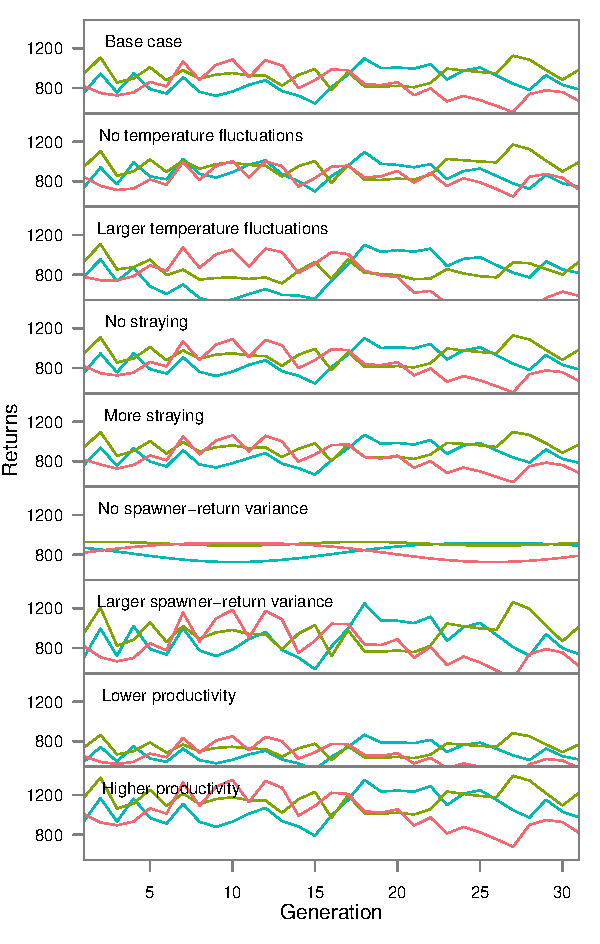
\includegraphics[width=4.0in]{../examples/figure/plot-various-options-ts-3pops.pdf}
\caption{The impact of increasing or decreasing various parameter values in the simulations. The different lines represent different salmon populations. (NEED TO ADD PARAMETER VALUES AND EXPAND THIS SLIGHTLY)}
\label{f:eg-sens}
\end{figure}

\clearpage

\begin{figure}[htbp]
\centering
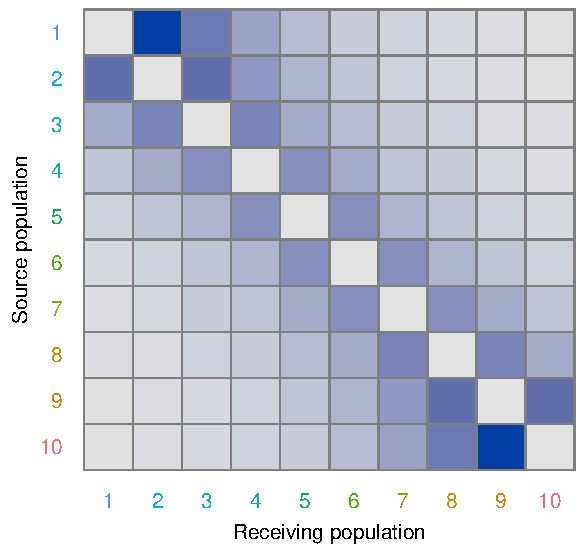
\includegraphics[width=4.0in]{../examples/figure/stray-matrix.pdf}
\caption{An example straying matrix. The rows and columns represent different 
populations (indicated by population number). Dark blue indicates a high rate 
of straying and light blue indicates a low rate of straying. The straying 
matrix is generated through equation \ref{eq:stray}.}
\label{f:stray}
\end{figure}

\clearpage

\begin{figure}[htbp]
\centering
\includegraphics[width=4.5in]{../examples/spatial-arma-sim.pdf}
\caption{Spatial and short-term environmental fluctuations}
\label{f:eg-sp-arma}
\end{figure}

\clearpage

\begin{figure}[htbp]
\centering
\includegraphics[width=4.5in]{../examples/spatial-linear-sim.pdf}
\caption{Spatial and long-term environmental fluctuations}
\label{f:eg-sp-linear}
\end{figure}

\clearpage

\begin{figure}[htbp]
\centering
\includegraphics[width=4.5in]{../examples/n-arma-sim.pdf}
\caption{Number and short-term environmental fluctuations}
\label{f:eg-n-arma}
\end{figure}

\clearpage

\begin{figure}[htbp]
\centering
\includegraphics[width=4.5in]{../examples/n-linear-sim.pdf}
\caption{Number and long-term environmental change}
\label{f:eg-n-linear}
\end{figure}

\clearpage

A placeholder: \citep{schindler2010}

\bibliographystyle{apalike}

\bibliography{jshort,som}


 %\end{spacing}

\end{document}


\clearpage

\section{Figure legends}

%\begin{center}
%\includegraphics[height=5.5in]{../examples/simulation-diagram3}
%\end{center}
%\textbf{Figure 1.} Flow chart of the salmon-metapopulation simulation. There are $n$ salmon populations and $t$ generations. Blue text indicates values that are generated before the simulation progresses through time. Red text indicates steps in which calculations are performed through time. Black text indicates values that are calculated. Grey text indicates parameters that can be set. Green text indicates the looping structure of the simulation.

%\clearpage

%\begin{center}
%\includegraphics[width=2.9in]{../examples/thermal-curve-scenarios}
%\end{center}
\textbf{Figure 1.} Different ways of prioritizing response-diversity conservation. Panel a shows thermal tolerance curves for ten possible populations and panels b--e show different ways of prioritizing four of those populations. The curves describe how productivity varies with temperature for a given population. Some populations thrive at low temperatures (cool colours) and some at warm temperatures (warm colours). Some are tolerant to a wider range of environmental conditions (yellow-to-green colours) but with a lower maximum productivity. The total possible productivity (the area under the curves) is the same for each population.

%\clearpage

%\begin{center}
%\includegraphics[width=4.0in]{../examples/spatial-arma-sim-full}
%\end{center}
%\textbf{Figure 3.} The components of an example metapopulation simulation. We show, from top to bottom, the temperature signal, the resulting productivity parameter (Ricker $a$), the salmon returns, fisheries catch, salmon escapement, salmon straying from their natal streams, salmon joining from other streams, spawner-return residuals on a log scale, and the estimated $a$ and $b$ parameters in the fitted Ricker curve. The colored lines indicate populations that thrive at low (cool colours) to high (warm colours) temperatures.

%\clearpage

%\begin{center}
%\includegraphics[width=4.5in]{../examples/spatial-mv}
%\end{center}
\textbf{Figure 2.} The importance of preserving environmental response diversity through spatial conservation strategies. The conservation strategies correspond to figure 2 and represent conserving a range of responses (green), the most stable populations only (orange), or one type of environmental response (purple and pink). In risk-return space we show environmental scenarios that are comprised primarily of (a) short-term and (b) long-term environmental fluctuations. The dots show simulated metapopulations and the contours show 25\% and 75\% quantiles across 500 simulations per strategy. We also show example metapopulation abundance time series for the (c, e) short-term and (d, f) long-term environmental-fluctuation scenarios. The grey line (a, b) indicates the efficient frontier across all simulated metapopulations --- metapopulations with the minimum variability for a given level of growth rate.

%\clearpage

%\begin{center}
%\includegraphics[width=4.5in]{../examples/cons-plans-n}
%\end{center}
\textbf{Figure 3.} The importance of preserving as many populations as possible when we don't know how response diversity is distributed. In risk-return space we show environmental scenarios that are comprised primarily of (a) short-term and (b) long-term environmental fluctuations. We show metapopulations in which 2 (red), 4 (orange), 8 (yellow), or 16 (green) populations of random response diversity are conserved. The dots show simulated metapopulations and the contours show 25\% and 75\% quantiles across 500 simulations per strategy. We also show example metapopulation (c) rate-of-change and (d) abundance time series for the short-term environmental-fluctuation scenario. The grey line (a, b) indicates the efficient frontier across all simulated metapopulations --- metapopulations with the minimum variability for a given level of growth rate.

\clearpage

\end{spacing}

%\setlength{\parskip}{8pt}
%\setlength{\parindent}{0cm}

 %\begin{spacing}{1.1}

 %\setcounter{page}{1}
 %\nolinenumbers
 %\section{Supporting online material}

\subsection{Supplementary code}

The \texttt{metafolio} \texttt{R} package and documentation.

\subsection{Supplementary figures}

\begin{figure}[htbp]
\centering
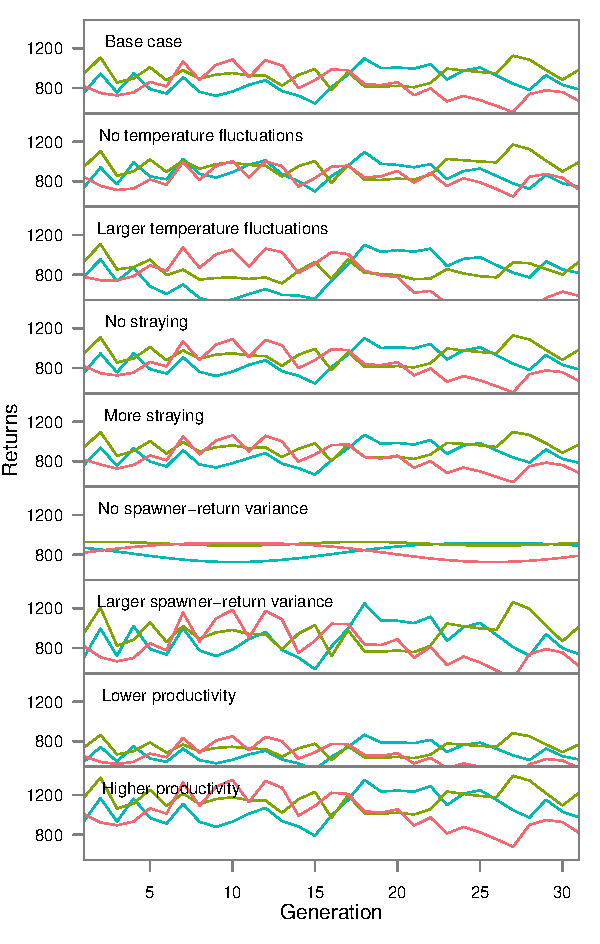
\includegraphics[width=4.0in]{../examples/figure/plot-various-options-ts-3pops.pdf}
\caption{The impact of increasing or decreasing various parameter values in the simulations. The different lines represent different salmon populations. (NEED TO ADD PARAMETER VALUES AND EXPAND THIS SLIGHTLY)}
\label{f:eg-sens}
\end{figure}

\clearpage

\begin{figure}[htbp]
\centering
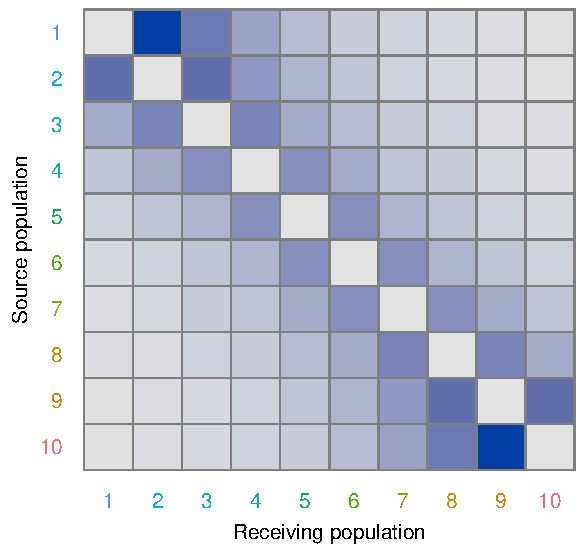
\includegraphics[width=4.0in]{../examples/figure/stray-matrix.pdf}
\caption{An example straying matrix. The rows and columns represent different 
populations (indicated by population number). Dark blue indicates a high rate 
of straying and light blue indicates a low rate of straying. The straying 
matrix is generated through equation \ref{eq:stray}.}
\label{f:stray}
\end{figure}

\clearpage

\begin{figure}[htbp]
\centering
\includegraphics[width=4.5in]{../examples/spatial-arma-sim.pdf}
\caption{Spatial and short-term environmental fluctuations}
\label{f:eg-sp-arma}
\end{figure}

\clearpage

\begin{figure}[htbp]
\centering
\includegraphics[width=4.5in]{../examples/spatial-linear-sim.pdf}
\caption{Spatial and long-term environmental fluctuations}
\label{f:eg-sp-linear}
\end{figure}

\clearpage

\begin{figure}[htbp]
\centering
\includegraphics[width=4.5in]{../examples/n-arma-sim.pdf}
\caption{Number and short-term environmental fluctuations}
\label{f:eg-n-arma}
\end{figure}

\clearpage

\begin{figure}[htbp]
\centering
\includegraphics[width=4.5in]{../examples/n-linear-sim.pdf}
\caption{Number and long-term environmental change}
\label{f:eg-n-linear}
\end{figure}

\clearpage

A placeholder: \citep{schindler2010}

\bibliographystyle{apalike}

\bibliography{jshort,som}


 %\end{spacing}

\end{document}

\begin{thebibliography}{64}
\expandafter\ifx\csname natexlab\endcsname\relax\def\natexlab#1{#1}\fi
\expandafter\ifx\csname url\endcsname\relax
  \def\url#1{{\tt #1}}\fi
\expandafter\ifx\csname urlprefix\endcsname\relax\def\urlprefix{URL }\fi

\bibitem[{Allendorf et~al.(1997)Allendorf, Bayles, Bottom, Currens, Frissell,
  Hankin, Lichatowich, Nehlsen, Trotter, and Williams}]{allendorf1997}
Allendorf, F.~W., D.~Bayles, D.~L. Bottom, K.~P. Currens, C.~A. Frissell,
  D.~Hankin, J.~A. Lichatowich, W.~Nehlsen, P.~C. Trotter, and T.~H. Williams.
\newblock 1997.
\newblock Prioritizing {Pacific} salmon stocks for conservation.
\newblock Conserv. Biol. 11:140--152.

\bibitem[{Anderson(2014)}]{metafoliopkg}
Anderson, S.~C. 2014.
\newblock metafolio: Salmon metapopulation simulations for conservation
  planning through portfolio optimization. R package version 0.1.0.
  http://cran.r-project.org/package=metafolio.

\bibitem[{Anderson et~al.(2013)Anderson, Cooper, and Dulvy}]{anderson2013}
Anderson, S.~C., A.~B. Cooper, and N.~K. Dulvy.
\newblock 2013.
\newblock Ecological prophets: Quantifying metapopulation portfolio effects.
\newblock Methods Ecol. Evol. 4:971--981.

\bibitem[{Ando and Mallory(2012)}]{ando2012}
Ando, A.~W., and M.~L. Mallory.
\newblock 2012.
\newblock Optimal portfolio design to reduce climate-related conservation
  uncertainty in the {Prairie Pothole Region}.
\newblock Proc. Natl. Acad. Sci. U.S.A. 109:6484--6489.

\bibitem[{Balvanera et~al.(2006)Balvanera, Pfisterer, Buchmann, He,
  Nakashizuka, Raffaelli, and Schmid}]{balvanera2006}
Balvanera, P., A.~B. Pfisterer, N.~Buchmann, J.-S. He, T.~Nakashizuka,
  D.~Raffaelli, and B.~Schmid.
\newblock 2006.
\newblock Quantifying the evidence for biodiversity effects on ecosystem
  functioning and services.
\newblock Ecol. Lett. 9:1146--1156.

\bibitem[{Battin et~al.(2007)Battin, Wiley, Ruckelshaus, Palmer, Korb, Bartz,
  and Imaki}]{battin2007}
Battin, J., M.~W. Wiley, M.~H. Ruckelshaus, R.~N. Palmer, E.~Korb, K.~K. Bartz,
  and H.~Imaki.
\newblock 2007.
\newblock Projected impacts of climate change on salmon habitat restoration.
\newblock Proc. Natl. Acad. Sci. U.S.A. 104:6720--6725.

\bibitem[{Beechie et~al.(2013)Beechie, Imaki, Greene, Wade, Wu, Pess, Roni,
  Kimball, Stanford, Kiffney, and Mantua}]{beechie2013}
Beechie, T., H.~Imaki, J.~Greene, A.~Wade, H.~Wu, G.~Pess, P.~Roni, J.~Kimball,
  J.~Stanford, P.~Kiffney, and N.~Mantua.
\newblock 2013.
\newblock Restoring salmon habitat for a changing climate.
\newblock River Res. Applic. 29:939--960.

\bibitem[{Carlson and Satterthwaite(2011)}]{carlson2011}
Carlson, S.~M., and W.~H. Satterthwaite.
\newblock 2011.
\newblock Weakened portfolio effect in a collapsed salmon population complex.
\newblock Can. J. Fish. Aquat. Sci. 68:1579--1589.

\bibitem[{Cooper and Mangel(1999)}]{cooper1999}
Cooper, A.~B., and M.~Mangel.
\newblock 1999.
\newblock The dangers of ignoring metapopulation structure for the conservation
  of salmonids.
\newblock Fish. Bull. 97:213--226.

\bibitem[{Crozier et~al.(2008)Crozier, Hendry, Lawson, Quinn, Mantua, Battin,
  Shaw, and Huey}]{crozier2008}
Crozier, L.~G., A.~P. Hendry, P.~W. Lawson, T.~Quinn, N.~J. Mantua, J.~Battin,
  R.~G. Shaw, and R.~B. Huey.
\newblock 2008.
\newblock Potential responses to climate change in organisms with complex life
  histories: evolution and plasticity in {Pacific} salmon.
\newblock Evol. Appl. 1:252--270.

\bibitem[{de~Mazancourt et~al.(2013)de~Mazancourt, Isbell, Larocque, Berendse,
  De~Luca, Grace, Haegeman, Wayne~Polley, Roscher, Schmid, Tilman, van Ruijven,
  Weigelt, Wilsey, and Loreau}]{demazancourt2013}
de~Mazancourt, C., F.~Isbell, A.~Larocque, F.~Berendse, E.~De~Luca, J.~B.
  Grace, B.~Haegeman, H.~Wayne~Polley, C.~Roscher, B.~Schmid, D.~Tilman, J.~van
  Ruijven, A.~Weigelt, B.~J. Wilsey, and M.~Loreau.
\newblock 2013.
\newblock Predicting ecosystem stability from community composition and
  biodiversity.
\newblock Ecol. Lett. 16:617--625.

\bibitem[{DFO(2005)}]{dfo2005wsp}
DFO. 2005.
\newblock Canada's policy for conservation of wild {Pacific} salmon.
\newblock Technical report, Fisheries and Oceans Canada, Vancouver, BC.

\bibitem[{Dorner et~al.(2008)Dorner, Peterman, and Haeseker}]{dorner2008}
Dorner, B., R.~M. Peterman, and S.~L. Haeseker.
\newblock 2008.
\newblock Historical trends in productivity of 120 {Pacific} pink, chum, and
  sockeye salmon stocks reconstructed by using a {Kalman} filter.
\newblock Can. J. Fish. Aquat. Sci. 65:1842--1866.

\bibitem[{Eliason et~al.(2011)Eliason, Clark, Hague, Hanson, Gallagher,
  Jeffries, Gale, Patterson, Hinch, and Farrell}]{eliason2011}
Eliason, E.~J., T.~D. Clark, M.~J. Hague, L.~M. Hanson, Z.~S. Gallagher, K.~M.
  Jeffries, M.~K. Gale, D.~A. Patterson, S.~G. Hinch, and A.~P. Farrell.
\newblock 2011.
\newblock Differences in thermal tolerance among sockeye salmon populations.
\newblock Science 332:109--112.

\bibitem[{Elmqvist et~al.(2003)Elmqvist, Folke, Nystr{\"o}m, Peterson,
  Bengtsson, Walker, and Norberg}]{elmqvist2003}
Elmqvist, T., C.~Folke, M.~Nystr{\"o}m, G.~Peterson, J.~Bengtsson, B.~Walker,
  and J.~Norberg.
\newblock 2003.
\newblock Response diversity, ecosystem change, and resilience.
\newblock Front. Ecol. Environ. 1:488--494.

\bibitem[{Figge(2004)}]{figge2004}
Figge, F.
\newblock 2004.
\newblock Bio-folio: applying portfolio theory to biodiversity.
\newblock Biodivers. Conserv. 13:827--849.

\bibitem[{Fraser et~al.(2011)Fraser, Weir, Bernatchez, Hansen, and
  Taylor}]{fraser2011}
Fraser, D.~J., L.~K. Weir, L.~Bernatchez, M.~M. Hansen, and E.~B. Taylor.
\newblock 2011.
\newblock Extent and scale of local adaptation in salmonid fishes: review and
  meta-analysis.
\newblock Heredity 106:404--420.

\bibitem[{Gustafson et~al.(2007)Gustafson, Waples, Myers, Weitkamp, Bryant,
  Johnson, and Hard}]{gustafson2007}
Gustafson, R.~G., R.~S. Waples, J.~M. Myers, L.~A. Weitkamp, G.~J. Bryant,
  O.~W. Johnson, and J.~J. Hard.
\newblock 2007.
\newblock Pacific salmon extinctions: quantifying lost and remaining diversity.
\newblock Conserv. Biol. 21:1009--1020.

\bibitem[{Haak and Williams(2012)}]{haak2012}
Haak, A.~L., and J.~E. Williams.
\newblock 2012.
\newblock Spreading the risk: native trout management in a warmer and
  less-certain future.
\newblock N. Am. J. Fish. Manage. 32:387--401.

\bibitem[{Hannah et~al.(2002)Hannah, Midgley, Lovejoy, Bond, Bush, Lovett,
  Scott, and Woodward}]{hannah2002a}
Hannah, L., G.~F. Midgley, T.~Lovejoy, W.~J. Bond, M.~Bush, J.~C. Lovett,
  D.~Scott, and F.~I. Woodward.
\newblock 2002.
\newblock Conservation of biodiversity in a changing climate.
\newblock Conserv. Biol. 16:264--268.

\bibitem[{Hilborn et~al.(2003)Hilborn, Quinn, Schindler, and
  Rogers}]{hilborn2003}
Hilborn, R.~W., T.~Quinn, D.~Schindler, and D.~Rogers.
\newblock 2003.
\newblock Biocomplexity and fisheries sustainability.
\newblock Proc. Natl. Acad. Sci. U.S.A. 100:6564--6568.

\bibitem[{Hilborn and Walters(1992)}]{hilborn1992}
Hilborn, R.~W., and C.~Walters.
\newblock 1992.
\newblock Quantitative Fisheries Stock Assessment: Choice, Dynamics, and
  Uncertainty.
\newblock Chapman and Hall, London.

\bibitem[{Isaak and Rieman(2013)}]{isaak2013}
Isaak, D.~J., and B.~E. Rieman.
\newblock 2013.
\newblock Stream isotherm shifts from climate change and implications for
  distributions of ectothermic organisms.
\newblock Global Change Biol. 19:742--751.

\bibitem[{Isaak et~al.(2007)Isaak, Thurow, Rieman, and Dunham}]{isaak2007}
Isaak, D.~J., R.~F. Thurow, B.~E. Rieman, and J.~B. Dunham.
\newblock 2007.
\newblock Chinook salmon use of spawning patches: relative roles of habitat
  quality, size, and connectivity.
\newblock Ecol. Appl. 17:352--364.

\bibitem[{Isaak et~al.(2012)Isaak, Wollrab, Horan, and Chandler}]{isaak2012}
Isaak, D.~J., S.~Wollrab, D.~Horan, and G.~Chandler.
\newblock 2012.
\newblock Climate change effects on stream and river temperatures across the
  northwest U.S. from 1980--2009 and implications for salmonid fishes.
\newblock Climatic Change 113:499--524.

\bibitem[{Ives and Carpenter(2007)}]{ives2007}
Ives, A.~R., and S.~R. Carpenter.
\newblock 2007.
\newblock Stability and diversity of ecosystems.
\newblock Science 317:58--62.

\bibitem[{Jentsch et~al.(2007)Jentsch, Kreyling, and
  Beierkuhnlein}]{jentsch2007}
Jentsch, A., J.~Kreyling, and C.~Beierkuhnlein.
\newblock 2007.
\newblock A new generation of climate-change experiments: events, not trends.
\newblock Front. Ecol. Environ. 5:365--374.

\bibitem[{Johnson and Schindler(2013)}]{johnson2013a}
Johnson, S.~P., and D.~E. Schindler.
\newblock 2013.
\newblock Marine trophic diversity in an anadromous fish is linked to its
  life-history variation in fresh water.
\newblock Biol. Lett. 9:20120824.

\bibitem[{Koellner and Schmitz(2006)}]{koellner2006}
Koellner, T., and O.~J. Schmitz.
\newblock 2006.
\newblock Biodiversity, ecosystem function, and investment risk.
\newblock BioScience 56:977--985.

\bibitem[{Lackey(2003)}]{lackey2003}
Lackey, R.~T.
\newblock 2003.
\newblock {Pacific Northwest} salmon: forecasting their status in 2100.
\newblock Rev. Fish. Sci. 11:35--88.

\bibitem[{Lee and Jetz(2008)}]{lee2008}
Lee, T.~M., and W.~Jetz.
\newblock 2008.
\newblock Future battlegrounds for conservation under global change.
\newblock Proc. R. Soc. Lond. B 275:1261--1270.

\bibitem[{Luce et~al.(2013)Luce, Abatzoglou, and Holden}]{luce2013}
Luce, C.~H., J.~T. Abatzoglou, and Z.~A. Holden.
\newblock 2013.
\newblock The missing mountain water: slower westerlies decrease orographic
  enhancement in the {Pacific Northwest USA}.
\newblock Science 342:1360--1364.

\bibitem[{Luce and Holden(2009)}]{luce2009}
Luce, C.~H., and Z.~A. Holden.
\newblock 2009.
\newblock Declining annual streamflow distributions in the {Pacific Northwest
  United States}, 1948--2006.
\newblock Geophys. Res. Lett. 36.

\bibitem[{Mantua et~al.(2010)Mantua, Tohver, and Hamlet}]{mantua2010}
Mantua, N., I.~Tohver, and A.~Hamlet.
\newblock 2010.
\newblock Climate change impacts on streamflow extremes and summertime stream
  temperature and their possible consequences for freshwater salmon habitat in
  {Washington State}.
\newblock Climatic Change 102:187--223.

\bibitem[{Margules and Pressey(2000)}]{margules2000}
Margules, C.~R., and R.~L. Pressey.
\newblock 2000.
\newblock Systematic conservation planning.
\newblock Nature 405:243--253.

\bibitem[{Markowitz(1952)}]{markowitz1952}
Markowitz, H.
\newblock 1952.
\newblock Portfolio Selection.
\newblock J. Finance 7:77--91.

\bibitem[{McClure et~al.(2008{\natexlab{{\em a\/}}})McClure, Carlson, Beechie,
  Pess, Jorgensen, Sogard, Sultan, Holzer, Travis, Sanderson, Power, and
  Carmichael}]{mcclure2008a}
McClure, M.~M., S.~M. Carlson, T.~J. Beechie, G.~R. Pess, J.~C. Jorgensen,
  S.~M. Sogard, S.~E. Sultan, D.~M. Holzer, J.~Travis, B.~L. Sanderson, M.~E.
  Power, and R.~W. Carmichael.
\newblock 2008{\natexlab{{\em a\/}}}.
\newblock Evolutionary consequences of habitat loss for {Pacific} anadromous
  salmonids.
\newblock Evol. Appl. 1:300--318.

\bibitem[{McClure et~al.(2008{\natexlab{{\em b\/}}})McClure, Utter, Baldwin,
  Carmichael, Hassemer, Howell, Spruell, Cooney, Schaller, and
  Petrosky}]{mcclure2008b}
McClure, M.~M., F.~M. Utter, C.~Baldwin, R.~W. Carmichael, P.~F. Hassemer,
  P.~J. Howell, P.~Spruell, T.~D. Cooney, H.~A. Schaller, and C.~E. Petrosky.
\newblock 2008{\natexlab{{\em b\/}}}.
\newblock Evolutionary effects of alternative artificial propagation programs:
  implications for viability of endangered anadromous salmonids.
\newblock Evol. Appl. 1:356--375.

\bibitem[{McCullough(1999)}]{mccullough1999}
McCullough, D.~A., 1999.
\newblock A review and synthesis of effects of alterations to the water
  temperature regime on freshwater life stages of salmonids, with special
  reference to {Chinook} salmon.
\newblock EPA 910-R-99-010, US Environmental Protection Agency.

\bibitem[{McElhany et~al.(2000)McElhany, Ruckelshaus, Ford, Wainwright, and
  Bjorkstedt}]{mcelhany2000}
McElhany, P., M.~H. Ruckelshaus, M.~J. Ford, T.~C. Wainwright, and E.~P.
  Bjorkstedt, 2000.
\newblock {Viable Salmonid Populations} and the recovery of {Evolutionarily
  Significant Units}.
\newblock Technical Report NOAA Tech. Memo. NMFS-NWFSC-42, U.S. Deptartment of
  Commerce.

\bibitem[{Moore et~al.(2010)Moore, Mcclure, Rogers, and Schindler}]{moore2010}
Moore, J.~W., M.~Mcclure, L.~A. Rogers, and D.~E. Schindler.
\newblock 2010.
\newblock Synchronization and portfolio performance of threatened salmon.
\newblock Conserv. Lett. 3:340--348.

\bibitem[{Mori et~al.(2013)Mori, Furukawa, and Sasaki}]{mori2013}
Mori, A.~S., T.~Furukawa, and T.~Sasaki.
\newblock 2013.
\newblock Response diversity determines the resilience of ecosystems to
  environmental change.
\newblock Biol. Rev. 88:349--364.

\bibitem[{Patterson et~al.(2007)Patterson, Skibo, Barnes, Hills, and
  Macdonald}]{patterson2007}
Patterson, D.~A., K.~M. Skibo, D.~P. Barnes, J.~A. Hills, and J.~S. Macdonald.
\newblock 2007.
\newblock The influence of water temperature on time to surface for adult
  sockeye salmon carcasses and the limitations in estimating salmon carcasses
  in the {Fraser River, British Columbia}.
\newblock N. Am. J. Fish. Manage. 27:878--884.

\bibitem[{Pestes et~al.(2008)Pestes, Peterman, Bradford, and Wood}]{pestes2008}
Pestes, L.~R., R.~M. Peterman, M.~J. Bradford, and C.~C. Wood.
\newblock 2008.
\newblock Bayesian decision analysis for evaluating management options to
  promote recovery of a depleted salmon population.
\newblock Conserv. Biol. 22:351--361.

\bibitem[{Policansky and Magnuson(1998)}]{policansky1998}
Policansky, D., and J.~J. Magnuson.
\newblock 1998.
\newblock Genetics, metapopulations, and ecosystem management of fisheries.
\newblock Ecol. Appl. 8:S119--S123.

\bibitem[{Pressey et~al.(2007)Pressey, Cabeza, Watts, Cowling, and
  Wilson}]{pressey2007}
Pressey, R.~L., M.~Cabeza, M.~E. Watts, R.~M. Cowling, and K.~A. Wilson.
\newblock 2007.
\newblock Conservation planning in a changing world.
\newblock Trends Ecol. Evolut. 22:583--592.

\bibitem[{Quinn(2005)}]{quinn2005}
Quinn, T.~P.
\newblock 2005.
\newblock The Behaviour and Ecology of Pacific Salmon and Trout.
\newblock American Fisheries Society, Bethesda, Maryland.

\bibitem[{{\textsf{R} Core Team}(2013)}]{r2013}
{\textsf{R} Core Team}, 2013.
\newblock \textsf{R}: {A} language and environment for statistical computing.
\newblock \textsf{R} Foundation for Statistical Computing, Vienna, Austria.

\bibitem[{Rogers and Schindler(2008)}]{rogers2008}
Rogers, L.~A., and D.~E. Schindler.
\newblock 2008.
\newblock Asynchrony in population dynamics of sockeye salmon in southwest
  {Alaska}.
\newblock Oikos 117:1578--1586.

\bibitem[{Ruckelshaus et~al.(2002)Ruckelshaus, Levin, Johnson, and
  Kareiva}]{ruckelshaus2002}
Ruckelshaus, M.~H., P.~Levin, J.~B. Johnson, and P.~M. Kareiva.
\newblock 2002.
\newblock The {Pacific} salmon wars: what science brings to the challenge of
  recovering species.
\newblock Annu. Rev. Ecol. Syst. 33:665--706.

\bibitem[{Scheuerell et~al.(2006)Scheuerell, Hilborn, Ruckelshaus, Bartz,
  Lagueux, Haas, and Rawson}]{scheuerell2006}
Scheuerell, M.~D., R.~Hilborn, M.~H. Ruckelshaus, K.~K. Bartz, K.~M. Lagueux,
  A.~D. Haas, and K.~Rawson.
\newblock 2006.
\newblock The {Shiraz} model: a tool for incorporating anthropogenic effects
  and fish--habitat relationships in conservation planning.
\newblock Can. J. Fish. Aquat. Sci. 63:1596--1607.

\bibitem[{Schindler et~al.(2008)Schindler, Augerot, Fleishman, Mantua, Riddell,
  Ruckelshaus, Seeb, and Webster}]{schindler2008}
Schindler, D.~E., X.~Augerot, E.~Fleishman, N.~J. Mantua, B.~Riddell,
  M.~Ruckelshaus, J.~Seeb, and M.~Webster.
\newblock 2008.
\newblock Climate change, ecosystem impacts, and management for {Pacific}
  salmon.
\newblock Fisheries 33:502--506.

\bibitem[{Schindler et~al.(2010)Schindler, Hilborn, Chasco, Boatright, Quinn,
  Rogers, and Webster}]{schindler2010}
Schindler, D.~E., R.~Hilborn, B.~Chasco, C.~P. Boatright, T.~P. Quinn, L.~A.
  Rogers, and M.~S. Webster.
\newblock 2010.
\newblock Population diversity and the portfolio effect in an exploited
  species.
\newblock Nature 465:609--612.

\bibitem[{Schtickzelle and Quinn(2007)}]{schtickzelle2007}
Schtickzelle, N., and T.~P. Quinn.
\newblock 2007.
\newblock A metapopulation perspective for salmon and other anadromous fish.
\newblock Fish Fish. 8:297--314.

\bibitem[{Stockwell et~al.(2003)Stockwell, Hendry, and
  Kinnison}]{stockwell2003}
Stockwell, C., A.~Hendry, and M.~Kinnison.
\newblock 2003.
\newblock Contemporary evolution meets conservation biology.
\newblock Trends. Ecol. Evol. 18:94--101.

\bibitem[{Thibaut et~al.(2012)Thibaut, Connolly, and Sweatman}]{thibaut2012}
Thibaut, L., S.~R. Connolly, and H.~P.~A. Sweatman.
\newblock 2012.
\newblock Diversity and stability of herbivorous fishes on coral reefs.
\newblock Ecology 93:891--901.

\bibitem[{Thomas(2010)}]{thomas2010}
Thomas, C.~D.
\newblock 2010.
\newblock Climate, climate change and range boundaries.
\newblock Divers. Distrib. 16:488--495.

\bibitem[{Thomas et~al.(2004)Thomas, Cameron, Green, Bakkenes, Beaumont,
  Collingham, Erasmus, de~Siqueira, Grainger, Hannah, Hughes, Huntley, van
  Jaarsveld, Midgley, Miles, Ortega-Huerta, Townsend~Peterson, Phillips, and
  Williams}]{thomas2004}
Thomas, C.~D., A.~Cameron, R.~E. Green, M.~Bakkenes, L.~J. Beaumont, Y.~C.
  Collingham, B.~F.~N. Erasmus, M.~F. de~Siqueira, A.~Grainger, L.~Hannah,
  L.~Hughes, B.~Huntley, A.~S. van Jaarsveld, G.~F. Midgley, L.~Miles, M.~A.
  Ortega-Huerta, A.~Townsend~Peterson, O.~L. Phillips, and S.~E. Williams.
\newblock 2004.
\newblock Extinction risk from climate change.
\newblock Nature 427:145--148.

\bibitem[{Thorson et~al.(2014{\natexlab{{\em a\/}}})Thorson, Jensen, and
  Zipkin}]{thorson2014a}
Thorson, J.~T., O.~P. Jensen, and E.~F. Zipkin.
\newblock 2014{\natexlab{{\em a\/}}}.
\newblock How variable is recruitment for exploited marine fishes? A
  hierarchical model for testing life history theory.
\newblock Can. J. Fish. Aquat. Sci. 71:973--983.

\bibitem[{Thorson et~al.(2014{\natexlab{{\em b\/}}})Thorson, Scheuerell, Buhle,
  and Copeland}]{thorson2014}
Thorson, J.~T., M.~D. Scheuerell, E.~R. Buhle, and T.~Copeland.
\newblock 2014{\natexlab{{\em b\/}}}.
\newblock Spatial variation buffers temporal fluctuations in early juvenile
  survival for an endangered {Pacific} salmon.
\newblock J. Anim. Ecol. 83:157--167.

\bibitem[{Walther et~al.(2002)Walther, Post, Convey, Menzel, Parmesan, Beebee,
  Fromentin, Hoegh-Guldberg, and Bairlein}]{walther2002}
Walther, G.-R., E.~Post, P.~Convey, A.~Menzel, C.~Parmesan, T.~J.~C. Beebee,
  J.-M. Fromentin, O.~Hoegh-Guldberg, and F.~Bairlein.
\newblock 2002.
\newblock Ecological responses to recent climate change.
\newblock Nature 416:389--395.

\bibitem[{Waples et~al.(2009)Waples, Beechie, and Pess}]{waples2009}
Waples, R., T.~Beechie, and G.~R. Pess.
\newblock 2009.
\newblock Evolutionary history, habitat disturbance regimes, and anthropogenic
  changes: what do these mean for resilience of {Pacific} salmon populations?
\newblock Ecol. Soc. 14:3.

\bibitem[{Winfree and Kremen(2009)}]{winfree2009}
Winfree, R., and C.~Kremen.
\newblock 2009.
\newblock Are ecosystem services stabilized by differences among species? {A}
  test using crop pollination.
\newblock Proc. R. Soc. Lond. B 276:229--237.

\bibitem[{Yeakel et~al.(2014)Yeakel, Moore, Guimar{\~a}es, and
  de~Aguiar}]{yeakel2014}
Yeakel, J.~D., J.~W. Moore, P.~R. Guimar{\~a}es, and M.~A.~M. de~Aguiar.
\newblock 2014.
\newblock Synchronisation and stability in river metapopulation networks.
\newblock Ecol. Lett. 17:272--283.

\end{thebibliography}

\clearpage

\section{Supplemental Material}

\noindent
\textsc{Appendix A.} The \texttt{metafolio} \textsf{R} package.

\noindent
\textsc{Appendix B.} Simulation input parameters and default values.

\noindent
\textsc{Appendix C.} An example straying matrix.

\noindent
\textsc{Appendix D.} Sensitivity illustration with alternative parameter values.

\noindent
\textsc{Appendix E.} An illustration of the correlation between populations.

\noindent
\textsc{Appendix F.} Example simulated time series from alternative conservation scenarios.

\clearpage

\section{Figure legends}

%\begin{center}
%\end{center}
\textsc{Fig. 1}. Flow chart of the salmon-metapopulation simulation.

%\clearpage

%\begin{center}
%\includegraphics[width=2.9in]{../examples/thermal-curve-scenarios}
%\end{center}
\bigskip
\noindent
\textsc{Fig. 2}. Different ways of prioritizing thermal-tolerance conservation. Panel a shows thermal-tolerance curves for ten possible populations and panels b--e show different ways of prioritizing four of those populations. The curves describe how productivity varies with temperature for a given population. Some populations thrive at low temperatures (light greys) and some at warm temperatures (dark greys). Some are tolerant to a wider range of environmental conditions (mid greys) but with a lower maximum productivity. The total possible productivity (the area under the curves) is the same for each population.

%\clearpage

%\begin{center}
%\includegraphics[width=4.0in]{../examples/spatial-arma-sim-full}
%\end{center}
\bigskip
\noindent
\textsc{Fig. \ref{f:ts}}. The components of an example metapopulation simulation. We show, from top to bottom, the temperature signal, the resulting productivity parameter (Ricker $a$), the salmon returns, fisheries catch, salmon escapement, salmon straying from their natal streams, salmon joining from other streams, spawner-return residuals on a log scale, and the estimated $a$ and $b$ parameters in the fitted Ricker curve. The shaded lines indicate populations that thrive at low (light grey) to high (dark grey) temperatures.

%\clearpage

%\begin{center}
%\includegraphics[width=4.5in]{../examples/spatial-mv}
%\end{center}
\bigskip
\noindent
\textsc{Fig. 4}. The importance of preserving thermal-tolerance diversity through spatial conservation strategies. The conservation strategies correspond to figure 2 and represent conserving a range of responses (green), the most stable populations only (orange), or one type of environmental response (purple and pink). In risk-return space we show environmental scenarios that are comprised primarily of (a) short-term and (b) long-term environmental fluctuations. The dots show simulated metapopulations and the contours show 25\% and 75\% quantiles across 500 simulations per strategy. We also show example metapopulation abundance time series for the (c, e) short-term and (d, f) long-term environmental-fluctuation scenarios. The thick grey line (a, b) indicates the efficient frontier across all simulated metapopulations --- metapopulations with the minimum variability for a given level of growth rate.

%\clearpage

%\begin{center}
%\includegraphics[width=4.5in]{../examples/cons-plans-n}
%\end{center}
\bigskip
\noindent
\textsc{Fig. 5}. The importance of preserving as many populations as possible when we do not know how thermal-tolerance is distributed. In risk-return space we show environmental scenarios that are comprised primarily of (a) short-term and (b) long-term environmental fluctuations. We show metapopulations in which two through 16 populations are conserved. The dots show simulated metapopulations and the contours show 25\% and 75\% quantiles across 500 simulations per strategy. We also show example metapopulation (c) rate-of-change and (d) abundance time series for the short-term environmental-fluctuation scenario. The thick grey line (a, b) indicates the efficient frontier across all simulated metapopulations --- metapopulations with the minimum variability for a given level of growth rate.

\bigskip
\noindent
\textsc{Fig. 6}. Risk-return trade-off in the case where habitat is lost over time through stream flow reduction. The temperature follows both short-term fluctuations and a long-term increase. Thermal tolerance is randomly conserved. Shading indicates conservation plans where two through 16 populations are conserved. (a) Conserving more populations decreases expected variance but also decreases expected growth rate. Dots show simulated metapopulations and contours show 25\% and 75\% quantiles across 500 simulations per strategy. The thick grey line indicates the efficient frontier across all simulated metapopulations --- metapopulations with the minimum variability for a given level of growth rate. Also shown are (b) example metapopulation growth rate and (c) abundance time series from the 2 and 16 population scenarios. Regression lines in (b) illustrate a decreasing growth rate through time.

\clearpage

\section{Figures}

\begin{center}
\includegraphics[height=5.5in]{Fig1}\\
\textsc{Fig.} 1
\clearpage
\includegraphics[width=2.4in]{Fig2}\\
\textsc{Fig.} 2
\clearpage
\includegraphics[width=4.2in]{Fig3}\\
\textsc{Fig.} 3
\clearpage
\includegraphics[width=4.5in]{Fig4}\\
\textsc{Fig.} 4
\clearpage
\includegraphics[width=4.5in]{Fig5}\\
\textsc{Fig.} 5
\clearpage
\includegraphics[width=3.0in]{Fig6}\\
\textsc{Fig.} 6
\clearpage
\end{center}

\end{spacing}

%\setlength{\parskip}{8pt}
%\setlength{\parindent}{0cm}

 \begin{spacing}{1.1}

 %\setcounter{page}{1}
 %\nolinenumbers
 %\section{Supporting online material}

\subsection{Supplementary code}

The \texttt{metafolio} \texttt{R} package and documentation.

\subsection{Supplementary figures}

\begin{figure}[htbp]
\centering
\includegraphics[width=4.0in]{../examples/figure/plot-various-options-ts-3pops.pdf}
\caption{The impact of increasing or decreasing various parameter values in the simulations. The different lines represent different salmon populations. (NEED TO ADD PARAMETER VALUES AND EXPAND THIS SLIGHTLY)}
\label{f:eg-sens}
\end{figure}

\clearpage

\begin{figure}[htbp]
\centering
\includegraphics[width=4.0in]{../examples/figure/stray-matrix.pdf}
\caption{An example straying matrix. The rows and columns represent different 
populations (indicated by population number). Dark blue indicates a high rate 
of straying and light blue indicates a low rate of straying. The straying 
matrix is generated through equation \ref{eq:stray}.}
\label{f:stray}
\end{figure}

\clearpage

\begin{figure}[htbp]
\centering
\includegraphics[width=4.5in]{../examples/spatial-arma-sim.pdf}
\caption{Spatial and short-term environmental fluctuations}
\label{f:eg-sp-arma}
\end{figure}

\clearpage

\begin{figure}[htbp]
\centering
\includegraphics[width=4.5in]{../examples/spatial-linear-sim.pdf}
\caption{Spatial and long-term environmental fluctuations}
\label{f:eg-sp-linear}
\end{figure}

\clearpage

\begin{figure}[htbp]
\centering
\includegraphics[width=4.5in]{../examples/n-arma-sim.pdf}
\caption{Number and short-term environmental fluctuations}
\label{f:eg-n-arma}
\end{figure}

\clearpage

\begin{figure}[htbp]
\centering
\includegraphics[width=4.5in]{../examples/n-linear-sim.pdf}
\caption{Number and long-term environmental change}
\label{f:eg-n-linear}
\end{figure}

\clearpage

A placeholder: \citep{schindler2010}

\bibliographystyle{apalike}

\bibliography{jshort,som}



 \end{spacing}

\end{document}
